\documentclass[a4paper, twoside, 11pt, czech, american]{book} % ASI template settings with 11pt instead of 12pt

%%% Packages:
%% Necessary packages:
\usepackage[T1]{fontenc}							% Font encoding
\usepackage[utf8]{inputenc}							% Input encoding
%\usepackage[a4paper, hmarginratio=3:2]{geometry}	% Use of the A4 page and setting the margins (the binding will be wider) ()
\usepackage[a4paper]{geometry}

%% Other packages:
% Code:
\usepackage{listings} 					% Code formatting package

% Fonts:
\usepackage{amsmath}  					% Advanced mathematic package
\usepackage{mathtools}					% Mathematics tools
\usepackage{xcolor}    					% Colorful text
\usepackage{soul}						% Text fonts syllable by syllable - used for in-text codifying
\usepackage[varg]{txfonts}				% Times New Roman fonts and math alphabets, for example, provides \mathbb{}
\usepackage{csquotes}					% Ensure that quoted texts are typeset according to the rules of the main language
\usepackage{microtype}					% Reduce text overflowing margins
\usepackage{xurl}						% URL formatting: better linebreaks in footnotes, etc.
\usepackage[shortcuts]{extdash} 		% Unbreakable dashes
\usepackage{tocloft}					% Dots in table of contents
\renewcommand\cftchapdotsep{\cftdotsep} % Dots in table of contents - activate
\usepackage{enumitem}					% Additional configuration of numbering in enumerate blocks. For example, item 1, subitem 1.1, etc.

% Format pages:
\usepackage{pdfpages}					% Add PDFs into compiled PDF

% Graphics:
\usepackage{float} 			  			% Advanced figure placement options
\usepackage{caption} 					% Captions of figures, tables, etc.
\usepackage{subcaption}					% Sub-captions of figures, tables, etc. 
\usepackage{tikz}						% Visual representation of matrices, graphs etc.
\usetikzlibrary{
	external,							% Externalize tikz pictures to avoid recompiling them with every compilation
	decorations.pathreplacing,			% Curly braces in tikz figures
	positioning,						% Advanced relative positioning
	shapes.arrows,						% Advanced arrow shapes
	arrows.meta,						% Advanced arrows
	calc								% Calculate point coordinates
}
\tikzexternalize[						% Add '-shell-escape' to the pdflatex compilation command. In TeXstudio: Options -> Configure Texstudio... -> Commands -> PdfLaTeX: 'pdflatex --synctex=1 -interaction=nonstopmode -shell-escape %.tex'
prefix=images/tikz/,				% Place externalized TikZ-generated images in a specific folder - ignored by git
optimize command away=\includepdf	% Optimize away including pdf pages to avoid compatibility issues of the 'pdfpages' package and the 'external' tikz library
]
\usepackage{pgfplots} 					% For visualizations, graphics, etc.
\pgfplotsset{compat=1.3}				% Use pgfplots version 1.3 specifically

% Languages:
\usepackage[czech, american]{babel}							 % Czech and American English are used in this document
\usepackage{silence}										 % Silence output of warnings
\WarningFilter{biblatex}{File 'american-iso.lbx' not found!} % Silence weird message that I couldn't find a solution for

% Referencing:
\usepackage{footmisc} 							 		  	% Refer to footnotes that already exist
\usepackage[
backend=biber,								  		  	% In TeXstudio, the backend here must correspond to: Options -> Configure TeXstudio... -> Build -> Default Bibliography Tool
style=iso-numeric,
sorting=none,
giveninits=true]{biblatex}								% Bibliography: ISO 690 format, cite shows numbers, sort according to occurrence in the text, shorten first names
\addbibresource{chapters/bibliography.bib}				  	% Specify path to bibliography file
\DeclareFieldFormat{labelnumberwidth}{\mkbibbrackets{#1}}	% Square brackets around numbers in the bibliography
\DeclareFieldFormat*{citetitle}{\mkbibemph{#1}}				% \citetitle{bibid} in text produces the title in emphasis for all sources. Without this, for example, the 'thesis' citation entry is non-emphasized with quotes while online sources are only emphasized (looks bad)
\setcounter{biburllcpenalty}{7000}						  	% Insert breakpoints after lowercase letters in URLs in the bibliography
\setcounter{biburlucpenalty}{8000}						  	% Insert breakpoints after uppercase letters in URLs in the bibliography

% Tables:
\usepackage{tabularx}			 % Advanced table options
\usepackage{colortbl} 			 % Table cell color

% Fonts (must be mentioned last to avoid warnings in the log)
\usepackage[hidelinks]{hyperref} % Hide square around URL link

%%% Document settings:
% TODO: Play around with the following if the formatting of pages turns out weird
\widowpenalty=9500 	   % Completely avoid widows (last lines of paragraph on a new page)
\clubpenalty=9500 	   % Completely avoid orphans (first lines of a new paragraph on the bottom of a page)
\brokenpenalty=9500    % Prohibit page breaks after a line that has a split word at the end

% ASI template settings
\topmargin=-15mm      % Top margin slightly smaller
\textwidth=150mm      % Width of text on the page
\textheight=240mm     % "Height" of text on the page

\pagenumbering{arabic} % Page numbering in Arabic numerals
\pagestyle{plain}      % Page numbering at the bottom center

\parindent=0pt 		   % Indentation of the 1st line of the paragraph
\parskip=7pt   		   % Space between paragraphs

\setlength{\emergencystretch}{20.0pt} % Allow compiler to create more spaces between words to avoid overflow of text


%%% Custom colors:
\definecolor{nvidia}{rgb}{0.6, 0.73, 0.35}		% Nvidia color
\definecolor{nvidia-light}{rgb}{0.92, 1.0, 0.85} % Nvidia light color
\definecolor{gray-light}{gray}{0.95}			% In-text code highlighting color
\definecolor{lbcolor}{rgb}{0.9,0.9,0.9}			% Code block background color
\definecolor{green-dark}{rgb}{0.0, 0.2, 0.13}	% Code block comments color


%%% Custom code block:
\lstset{
	backgroundcolor=\color{lbcolor}, % Background color of the code block
	upquote=true,					 % Format of quote: true -> '', false -> ‘’
	columns=fixed,					 % Characters are below each other (each column is one character -> fixed column size)
	extendedchars=false,			 % Allow national characters, for example, Czech diacritics. If true, then load any package that defines the characters, for example, fontenc, or inputenc, etc.
	showtabs=false,					 % Tabulators visible or not
	showspaces=false,				 % All blank spaces visible as _ or not
	showstringspaces=false,			 % Blank spaces in strings visible as _ or not 
	identifierstyle=\ttfamily,		 % Code font to be monospace if the line begins with one of the following: a-z, A-Z, @, $ and _
	language=C++,					 % Default language syntax highlighting for code blocks
	captionpos=b,					 % Position of the caption. b - bottom; t - top of the listing
	tabsize=2,						 % Set tabulator stops			
	frame=lines,					 % Draw a line on the top and bottom of the code listing -> frame
	numbers=left,					 % Print line numbers on the left of the code block
	numberstyle=\tiny,				 % Font and size of line numbers
	numbersep=5pt,					 % Distance between line numbers and the code block
	basicstyle=\footnotesize,		 % Basic font. Selected at the beginning of each listing
	keywordstyle=\color[rgb]{0,0,1}, % Fond of language keywords in a specific font
	commentstyle=\color{green-dark}, % Font of comments in code block
	stringstyle=\color{red},		 % Font of non-keywords, comments and strings
	breaklines=true,				 % Breaking of long lines
	prebreak = \raisebox{0ex}[0ex][0ex]{\ensuremath{\hookleftarrow}}, % Line-break symbol if a line of code is too long
}
% Extend C++ with CUDA keywords - not supported in lstlisting by default.
\lstset{
	morekeywords={__global__},
	morekeywords={__device__},
	morekeywords={blockDim.x},
	morekeywords={blockDim.y},
	morekeywords={blockIdx.x},
	morekeywords={blockIdx.y},	
	morekeywords={threadIdx.x},
	morekeywords={threadIdx.y},
	morekeywords={gridDim.x},
	morekeywords={__shared__},
	morekeywords={dim3},
	alsoletter={.}			   % Make the font be applied for dots
}


%%% Custom math operators:
\DeclareMathOperator*{\argmax}{arg\,max}
\DeclareMathOperator*{\argmin}{arg\,min}
\DeclarePairedDelimiter\parens{\lparen}{\rparen}
\newcommand{\minp}[1]{\min\parens*{#1}}

%%% Custom commands:
\newcommand{\ti}{\textit} 								  									   % Shortcut for cursive font
\newcommand{\tb}{\textbf} 								  									   % Shortcut for bold fond
\DeclareRobustCommand{\code}[1]{{\begingroup\sethlcolor{gray-light}\hl{\texttt{#1}}\endgroup}} % Shortcut for code font in text
\soulregister{\code}{1}																		   % Codeify inline text character by character

%% Status of writing:
\newcommand{\TODO}{\textcolor{red}{TODO}}   		   % To-Do command
\newcommand{\TO}{\textcolor{nvidia}{TO}} 			   % Writing to-be checked by the supervisor (Tomas Oberhuber)


%%% Constants
\newcommand{\cvut}{České vysoké učení technické v Praze}
\newcommand{\fjfi}{Fakulta jaderná a fyzikálně inženýrská}
\newcommand{\ksi}{Katedra softwarového inženýrství}
\newcommand{\programme}{Aplikace přírodních věd}
\newcommand{\specialization}{Aplikace softwarového inženýrství}

\newcommand{\kind}{Diplomová práce}

\newcommand{\logoCVUT}{
\includegraphics{images/title/cvut_logo_contour_version.pdf}}

% The following was filled in accordance with the original task paper
\newcommand{\titleCZ}{Paralelní výpočet LU rozkladu na GPU pro numerické řešení parciálních diferenciálních rovnic}					 % Czech title of the project
\newcommand{\titleEN}{Parallel Computation of LU Decomposition on GPUs for the Numerical Solution of Partial Differential Equations} % English title of the project
\newcommand{\paperAuthor}{Bc. Lukáš Čejka}   				 % Name and surname, including academic titles
\newcommand{\supervisor}{doc. Ing. Tomáš Oberhuber, Ph.D.} 	 % Name and surname of supervisor, including academic titles
\newcommand{\supervisorWorkspace}{\ksi, \fjfi, \cvut} 		 % Workplace of supervisor

\newcommand{\consultant}{--} 								 % Consultant's name, surname and academic titles, if I have a consultant
\newcommand{\consultantWorkspace}{--} 						 % Consultant's workplace, if I have a consultant

\newcommand{\yearSubmitted}{2023}  							 % Year of handing in the thesis (not the academic years)
\newcommand{\place}{Praze} 									 % City of studying

\newcommand{\keywordCZ}{\TODO}
\newcommand{\keywordEN}{\TODO}
\newcommand{\abstractCZ}{\TODO}
\newcommand{\abstractEN}{\TODO}

% Declaration in Czech
\newcommand{\declarationCZ}{Prohlašuji, že jsem svou diplomovou práci vypracoval samostatně a použil jsem pouze podklady (literaturu, projekty, SW atd.) uvedené v přiloženém seznamu.}

% Declaration in English (translation of the Czech declaration)
\newcommand{\declarationEN}{I declare that I have carried out my Master's Degree Project independently and I have used only the materials (literature, projects, software, etc.) listed in the bibliography.}

% Acknowledgement in Czech
\newcommand{\acknowledgementCZ}{Chtěl bych poděkovat doc. Ing. Tomáši Oberhuberovi, Ph.D. za vedení mé diplomové práce a za podnětné návrhy, které ji obohatily. Poděkování patří také zpřístupnění výpočetní infrastruktury projektu financovaného OP VVV CZ.02.1.01/0.0/0.0/16\_019/0000765 ``Výzkumné centrum informatiky''.}

% Acknowledgement in English (translation of the Czech acknowledgement)
\newcommand{\acknowledgementEN}{I would like to thank doc. Ing. Tomas Oberhuber, Ph.D. for supervising my master's thesis and for the inspiring proposals that enriched it. The access to the computational infrastructure of the OP VVV funded project CZ.02.1.01/0.0/0.0/16\_019/0000765 ``Research Center for Informatics'' is also gratefully acknowledged.}




\begin{document}
\shorthandoff{-} % This prevents issues with the 'czech' package: https://tex.stackexchange.com/questions/477449/incomplete-iffalse-related-listlisting-textit-and-textcolor




%%%%%%%%%%%% TITLE PAGE %%%%%%%%%%%%
\thispagestyle{empty}
\selectlanguage{czech}%

\begin{center}
	{\LARGE
		\cvut\par
		\fjfi
	}
	\vspace{10mm}
	
	\begin{tabular}{c}
		\textbf{\ksi} \\[3pt]   
		\textbf{Obor: \specialization}\\
	\end{tabular}
	
	\vspace{10mm} \logoCVUT \vspace{15mm} 
	
	{\huge \textbf{\titleCZ}\par}
	\vspace{5mm}
	\selectlanguage{american}%
	{\huge \textbf{\titleEN}\par}
	\selectlanguage{czech}%
	
	\vspace{15mm}
	{\Large \MakeUppercase{\kind}}
	
	\vfill
	{\large
		\begin{tabular}{ll}
			Vypracoval: & \paperAuthor\\
			Vedoucí práce: & \supervisor\\
			Rok: & \yearSubmitted
		\end{tabular}
	}
\end{center}

\clearpage{\pagestyle{empty}\cleardoublepage} % Empty page after the title page - no numbering




%%%%%%%%%%%% TASK PAPER %%%%%%%%%%%%
\newpage  			  % DO NOT TOUCH!
\thispagestyle{empty} % DO NOT TOUCH!

% Task paper scanned as a 2-page PDF:
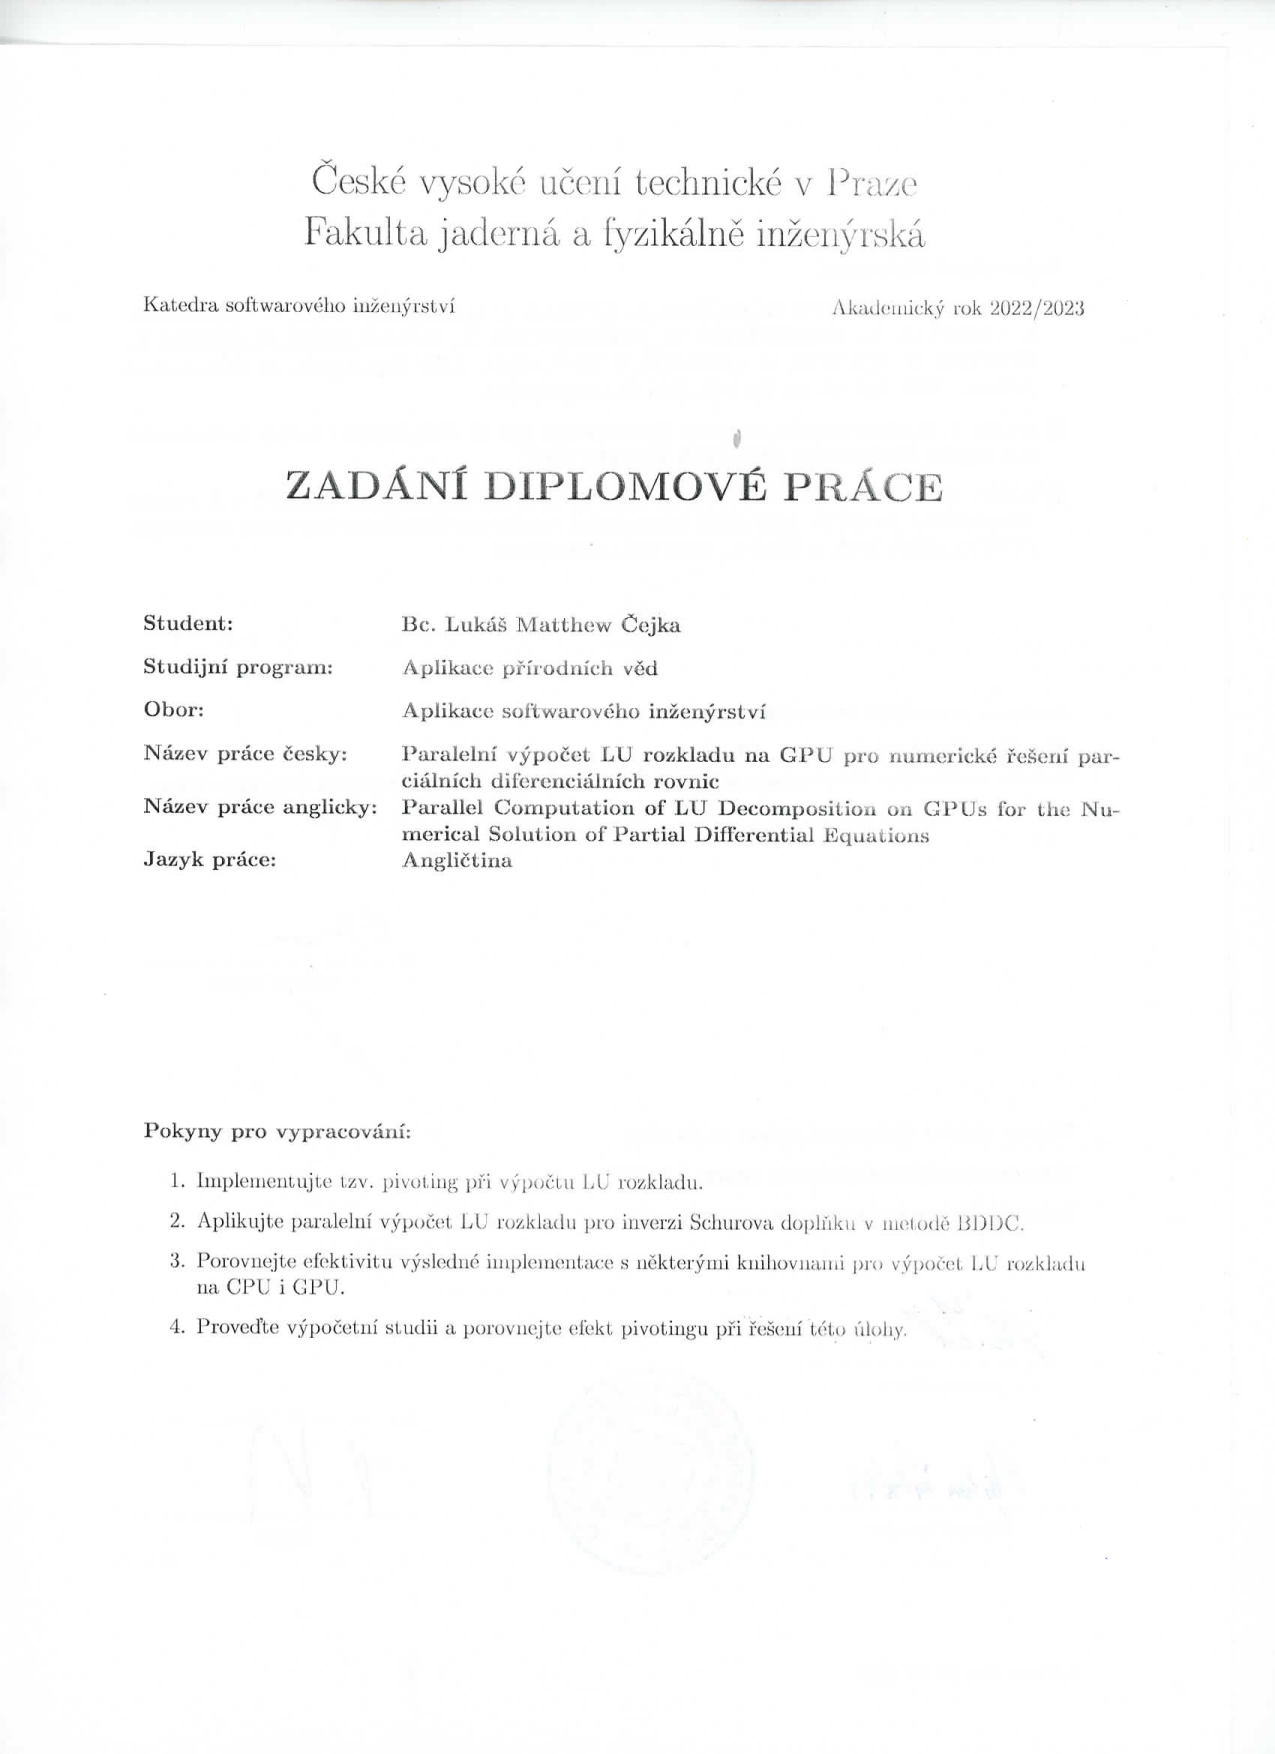
\includepdf[pages={1, 2}]{resources/masters_thesis_assignment_lukas_matthew_cejka.pdf}
%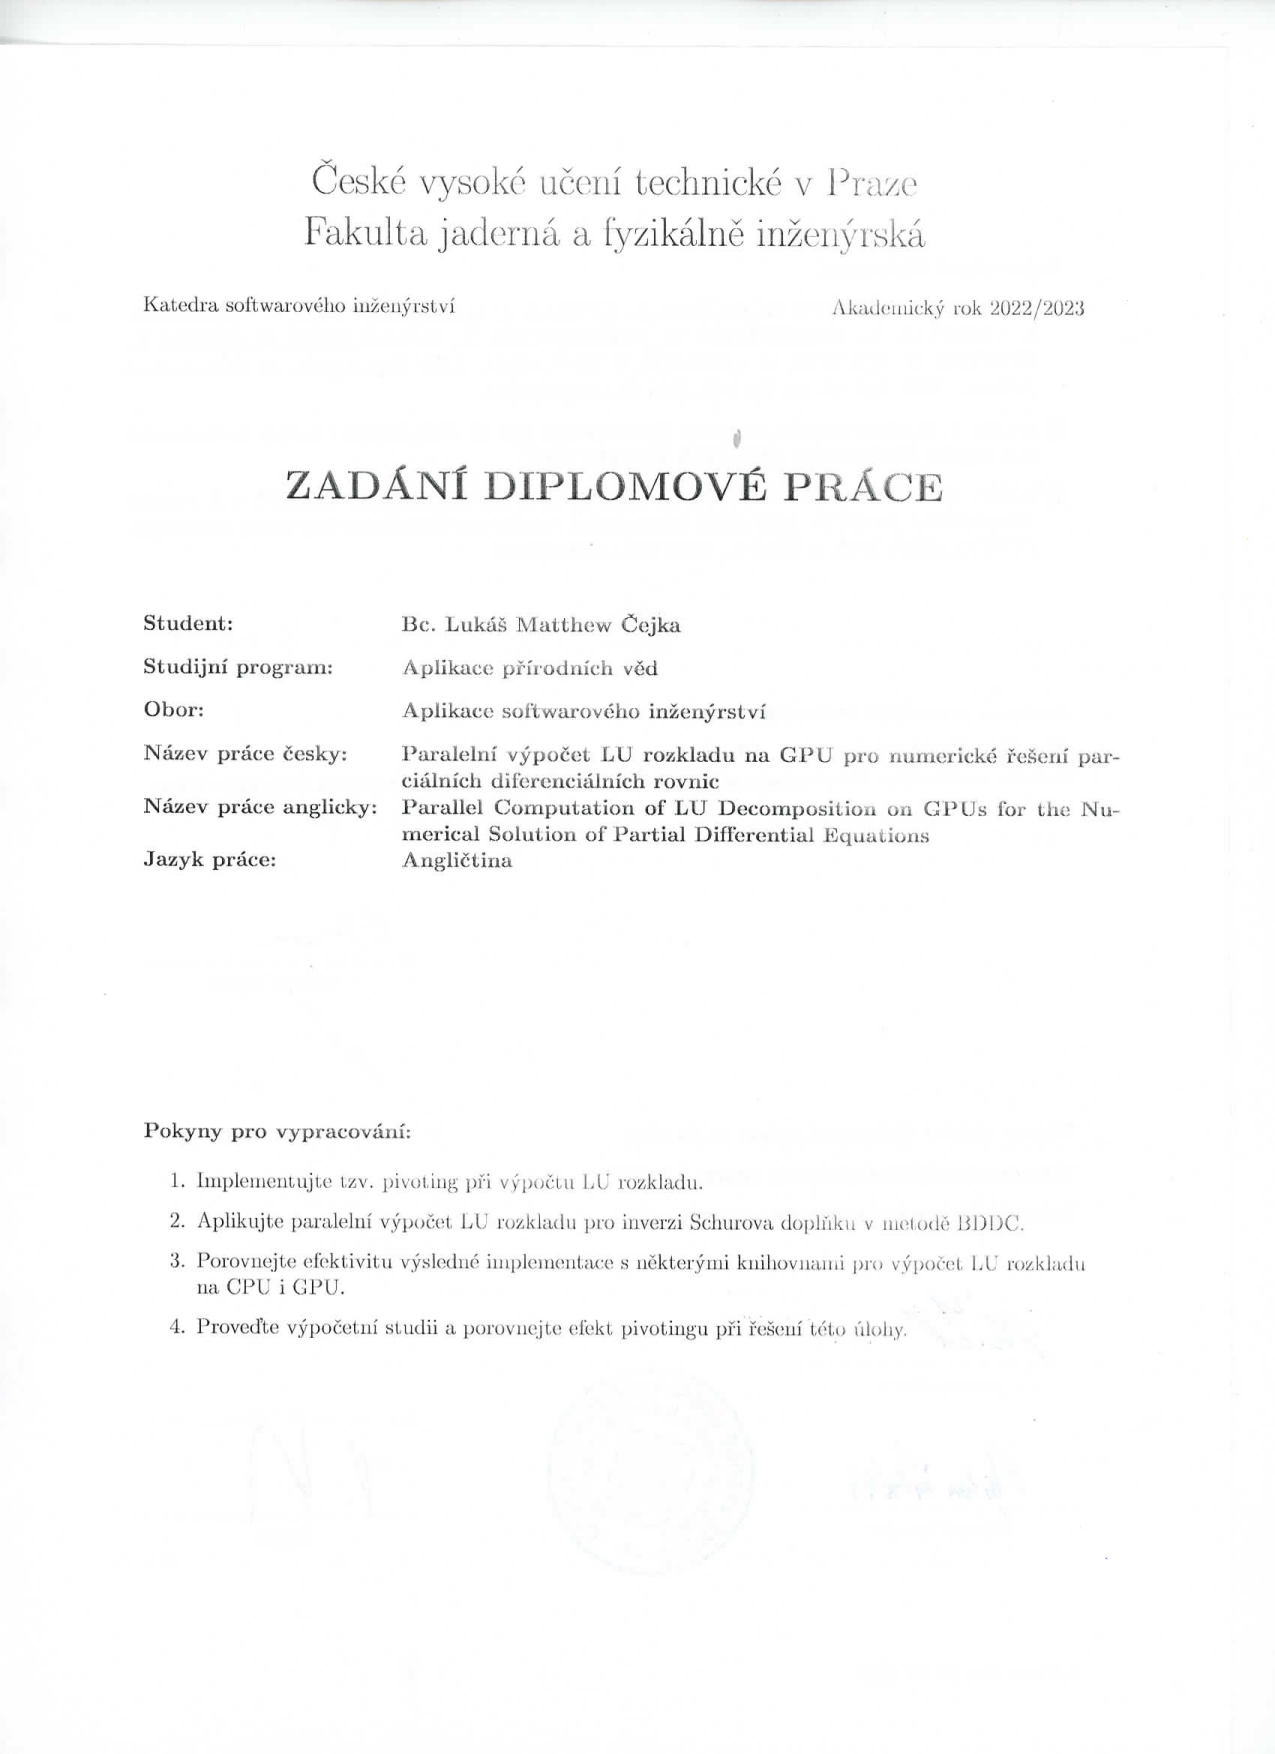
\includegraphics{resources/masters_thesis_assignment_lukas_matthew_cejka.pdf}




%%%%%%%%%%%% DECLARATION %%%%%%%%%%%%
\newpage 			  % DO NOT TOUCH!
\thispagestyle{empty} % DO NOT TOUCH!

~ 					  % DO NOT TOUCH!
\vfill 				  % Empty fill. DO NOT TOUCH!

\textbf{Prohlášení}   % DO NOT TOUCH!

\vspace{1em} 		  % DO NOT TOUCH!
\declarationCZ

\selectlanguage{american}%
\vspace{1em}
\textbf{Declaration}

\vspace{1em}
\declarationEN
\selectlanguage{czech}%

\vspace{2em}  									 							    	% DO NOT TOUCH!
\hspace{-0.5em}\begin{tabularx}{\textwidth}{X c} 							    	% DO NOT TOUCH!
	V \place\ dne .................... &........................................ \\ % DO NOT TOUCH!
	& \paperAuthor
\end{tabularx}




%%%%%%%%%%%% ACKNOWLEDGEMENT  %%%%%%%%%%%%
\newpage
\thispagestyle{empty}

~
\vfill % Empty fill

\textbf{Poděkování}

\vspace{1em} 				% Vertical space. % DO NOT TOUCH!
\acknowledgementCZ

\selectlanguage{american}%
\vspace{1em}
\textbf{Acknowledgment}

\selectlanguage{czech}%
\vspace{1em} 				% Vertical space. % DO NOT TOUCH!
\acknowledgementEN
\begin{flushright}
	\paperAuthor
\end{flushright}  			% Acknowledgement page ends here




%%%%%%%%%%%% ABSTRACT %%%%%%%%%%%% 
\newpage   			  % DO NOT TOUCH!
\thispagestyle{empty} % DO NOT TOUCH!

% Preparation: DO NOT TOUCH the next 8 lines!
\newbox\odstavecbox
\newlength\vyskaodstavce
\newcommand\odstavec[2]{%
	\setbox\odstavecbox=\hbox{%
		\parbox[t]{#1}{#2\vrule width 0pt depth 4pt}}%
	\global\vyskaodstavce=\dp\odstavecbox
	\box\odstavecbox}
\newcommand{\delka}{120mm} % Text width in 2nd table column

% Using the preparation: DO NOT TOUCH commands inside the "tabular" section!
\begin{tabular}{ll}
	{\em Název práce:} & ~ \\
	\multicolumn{2}{l}{\odstavec{\textwidth}{\bf \titleCZ}} \\[1em]
	{\em Autor:} & \paperAuthor \\[1em]
	{\em Studijní program:} & \programme \\
	{\em Obor:} & \specialization \\
	{\em Druh práce:} & \kind \\[1em]
	{\em Vedoucí práce:} & \odstavec{\delka}{\supervisor\\ \supervisorWorkspace} \\
	{\em Konzultant:} & -- %\odstavec{\delka}{\consultant \\ \consultantWorkspace}  % TODO: Remove the text "-- %" if you had a consultant
	\\[1em]  
	\multicolumn{2}{l}{\odstavec{\textwidth}{{\em Abstrakt:} ~ \abstractCZ  }} \\[1em]
	{\em Klíčová slova:} & \odstavec{\delka}{\keywordCZ} \\[2em]
	\selectlanguage{american}%
	{\em Title:} & ~\\
	\multicolumn{2}{l}{\odstavec{\textwidth}{\bf \titleEN}}\\[1em]
	{\em Author:} & \paperAuthor \\[1em]
	\multicolumn{2}{l}{\odstavec{\textwidth}{{\em Abstract:} ~ \abstractEN  }} \\[1em]
	{\em Key words:} & \odstavec{\delka}{\keywordEN}
\end{tabular}




%%%%%%%%%%%% CONTENTS OF THE PAPER %%%%%%%%%%%%
\selectlanguage{american}%
\newpage  		 % DO NOT TOUCH!
\parskip=0pt
\tableofcontents % DO NOT TOUCH!
\parskip=7pt
\newpage 		 % DO NOT TOUCH!




%--------------------------------------------------------
%|         The PAPER ITSELF begins here                 |
%--------------------------------------------------------

\chapter*{Nomenclature}		 		 		 % DO NOT TOUCH!
\addcontentsline{toc}{chapter}{Nomenclature} % DO NOT TOUCH!

\begin{table}[ht]
	\begin{tabular}{l|l}
		\hline
		Abbreviation  & Meaning                                                             \\ \hline
		CPU			  & Central Processing Unit                                             \\
		GPU			  & Graphics Processing Unit                                            \\
		SIMT		  & Single-Instruction Multiple-Thread                                  \\
		SIMD		  & Single-Instruction Multiple-Data                                    \\
		CM            & Crout Method                                                        \\
		CMPP          & Crout Method with Partial Pivoting                                 	\\
		ICMPP         & Iterative Crout Method with Partial Pivoting                        \\
		PCM           & Parallel Crout Method                                               \\
		PCM\textit{x} & Parallel Crout Method that uses 1D thread blocks of x threads       \\
		ICM           & Iterative Crout Method                                              \\
		ICM\textit{x} & Iterative Crout Method that uses 2D thread blocks of x by x threads \\
		IS            & Iterative Solver                                                    \\
		IS\textit{x}  & Iterative Solver that uses 1D thread blocks of x threads            \\
		HPC           & High-Performance Computing                                          \\
		LUP           & Lower-Upper decomposition with partial Pivoting                     \\ \hline
	\end{tabular}
	\caption{Abbreviations used in this project.}
	\label{Table:nomenclature}
\end{table}

\chapter*{Introduction}		 		 		 % DO NOT TOUCH!
\addcontentsline{toc}{chapter}{Introduction} % DO NOT TOUCH!

\TODO

\chapter{Theory}

This chapter will introduce the theory behind the core parts of this project.
First, Nvidia's Graphics Processing Units (GPUs) and their use in General-Purpose Computing on GPUs (GPGPU) will be briefly described.
Then, CUDA, the API for communicating with Nvidia GPUs, will be presented.
The final part introduces the method implemented in this project: Iterative Crout's Method with Partial Pivoting (ICMPP).

\section{GPUs}\label{Section:theory->GPUs}
In essence, a Graphics Processing Unit (GPU) is a device designed to accelerate the graphical output of a computer system.
Simply put, a GPU comprises many smaller processing units.
While these units are not as fast as the cores of a CPU, they excel at processing many similar tasks in parallel.
An example of such a task is displaying an image on a monitor.
In simple terms, to display the image, each pixel must be computed and rendered.
If the image is 1,200 by 1,200 pixels, then, the processing entity must compute and render 1,440,000 individual points.
Given the many processing units that the GPU has, it is capable of performing this operation efficiently.

While the common understanding of a GPU is that it is an image-processing device, how it processes images can be leveraged for non-graphical computation-heavy tasks.
This is referred to as General-Purpose Computing on Graphics Processing Units (GPGPU).

\subsection{General-Purpose Computing on Graphics Processing Units (GPGPU)}\label{Subsection:theory->GPUs->GPGPU}
General-Purpose Computing on Graphics Processing Units (GPGPU) has become an integral part of High-Performance Computing (HPC) in the last two decades \cite{Cejka2020, Cejka2022}.
One of the key parts of GPGPU is to tailor tasks for efficient execution on GPUs.
To use a GPU efficiently, it is necessary to parallelize the workload.
A common example of a parallelizable task is the multiplication of two matrices.
Without parallelism and assuming the naive matrix-multiplication algorithm, this task requires the processing entity to perform the pseudocode shown in Listing~\ref{Listing:theory->GPUs->GPGPUs->multiplication-of-matrices}.

\begin{lstlisting}[caption={Pseudocode for the multiplication of two matrices.
Let $\mathbf{A}$ be a $m\times n$ matrix, $\mathbf{B}$ a $n\times p$ matrix, and $\mathbf{C}$ a $m\times p$ matrix.},label={Listing:theory->GPUs->GPGPUs->multiplication-of-matrices}]
multiplyMatrices(A, B, C):
	for i from 0 to m - 1:
		for j from 0 to p - 1:
			for k from 0 to n - 1:
				C[i, j] += A[i, k] * B[k, j]
\end{lstlisting}

Since parallelism is not used, the computation is strictly sequential and would arguably benefit from the faster core clock speeds of a CPU \cite{Cejka2022}.
However, since the computation of every element in $\mathbf{C}$ is independent of the other elements, it is possible to compute all elements of $\mathbf{C}$ simultaneously.
In other words, every thread of the GPU can be tasked to compute one element of $\mathbf{C}$, i.e., each thread would only compute the innermost loop.\\
Note that the parallelization of certain tasks is not as straightforward, for example, Crout Method with partial pivoting (detailed in Section~\ref{Subsection:theory->ICMPP->LUP->CMPP}).

Similarly to the above-mentioned example of displaying the image on a monitor, the GPU - and its many processing units - greatly benefits from the parallelized workload largely due to its architecture.
To illustrate this, Figure~\ref{Figure:theory->GPUs->GPGPU->CPU-nvidia-GPU-architecture-comparison} shows a general architecture comparison of a CPU and a GPU.

\begin{figure}[ht!]
	\centering
	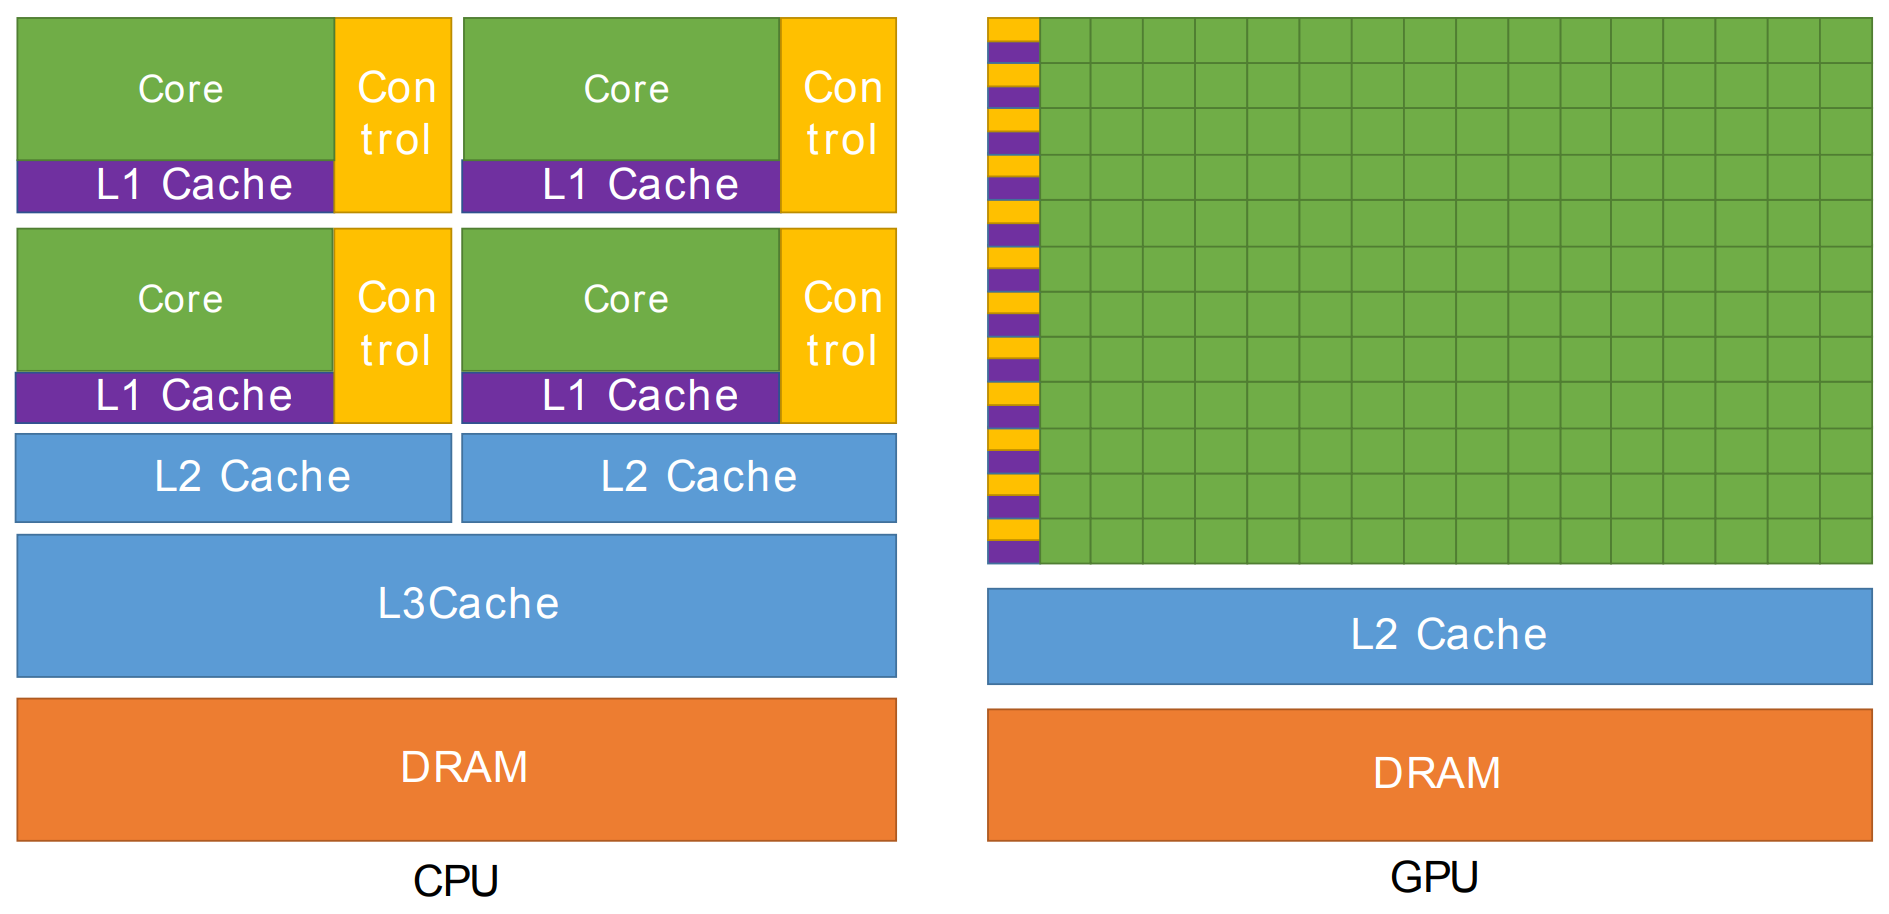
\includegraphics[width=14cm, keepaspectratio]{images/ch01/nvidia_CPU_GPU_comparison.png}
	\caption{Architecture comparison of a CPU and a GPU.
		Taken from \citetitle{NVIDIADecember2022} \cite{NVIDIADecember2022}.
	}
	\label{Figure:theory->GPUs->GPGPU->CPU-nvidia-GPU-architecture-comparison}
\end{figure}

In Figure~\ref{Figure:theory->GPUs->GPGPU->CPU-nvidia-GPU-architecture-comparison} it can be seen that the control units and caches of the CPU are proportionately sized to illustrate that GPUs do not focus on fine-grained cache control and prediction logic as much as CPUs.
The reasoning behind this is that CPUs in general attempt to use the aforementioned focus points to hide memory latency.
On the other hand, GPUs do not attempt to hide memory latency with controllers using costly caching.
Instead, as mentioned in \citetitle{NVIDIADec2022} \cite{NVIDIADec2022}, it is considered best practice for the developer to hide memory latency using CUDA-specific functionalities \cite{Sanglard2May2020}.

In Nvidia GPUs, the control units are referred to as Stream Multiprocessors (SMs) and they are responsible for scheduling tasks to processing units.
Therefore, it can be argued that the computational power of an Nvidia GPU depends on - among other factors - the number of SMs it has and their capabilities.
The reasoning behind this is that the more SMs a GPU has, the more concurrent computations it is capable of performing.
To exemplify this, see Table~\ref{Table:theory->GPUs->GPGPU->nvidia-gpu-details-comparison} for a selection of the latest Nvidia Datacenter cards and their relevant specifications.

\begin{table}[ht!]
	\centering
	\renewcommand{\arraystretch}{0.9}
	\begin{tabular}{|>{\raggedright\arraybackslash\bfseries\scriptsize}m{2.7cm}|>{\scriptsize}m{2.7cm}|>{\scriptsize}m{2.7cm}|>{\scriptsize}m{2.7cm}|}
		\hline
		\rowcolor{nvidia}\multicolumn{1}{|>{\centering\arraybackslash\normalsize}m{2.72cm}|}{$\vcenter{\textbf{GPU Features}}$} 
		& \multicolumn{1}{>{\centering\arraybackslash\normalsize}m{2.72cm}|}{$\vcenter{\textbf{V100}}$}
		& \multicolumn{1}{>{\centering\arraybackslash\normalsize}m{2.72cm}|}{$\vcenter{\textbf{A100}}$}
		& \multicolumn{1}{>{\centering\arraybackslash\normalsize}m{2.72cm}|}{$\vcenter{\textbf{H100}}$}\\[5pt]
		\hline
		GPU & GV100 (Volta) & GA100 (Ampere) & GH100 (Hopper) \\
		\hline
		GPU Board Form Factor & SXM2 & SXM4 & SXM5 \\
		\hline
		\rowcolor{nvidia-light}\multicolumn{1}{|>{\arraybackslash\bfseries\scriptsize}m{2.72cm}|}{SMs}
		& \multicolumn{1}{>{\arraybackslash\scriptsize}m{2.72cm}|}{80}
		& \multicolumn{1}{>{\arraybackslash\scriptsize}m{2.72cm}|}{108}
		& \multicolumn{1}{>{\arraybackslash\scriptsize}m{2.72cm}|}{132} \\
		\hline
		FP32 Cores / SM & 64 & 64 & 128 \\
		\hline
		FP32 Cores / GPU & 5,120 & 6,912 & 16,896 \\
		\hline
		FP64 Cores / SM & 32 & 32 & 64 \\
		\hline
		FP64 Cores / GPU & 2,560 & 3,456 & 8,448 \\
		\hline
		GPU Boost Clock & 1,530 MHz & 1,410 MHz & 1,830 MHz \\
		\hline
		\rowcolor{nvidia-light}\multicolumn{1}{|>{\arraybackslash\bfseries\scriptsize}m{2.72cm}|}{Peak FP32 TFLOPS}
		& \multicolumn{1}{>{\arraybackslash\scriptsize}m{2.72cm}|}{15.7}
		& \multicolumn{1}{>{\arraybackslash\scriptsize}m{2.72cm}|}{19.5}
		& \multicolumn{1}{>{\arraybackslash\scriptsize}m{2.72cm}|}{66.9} \\
		\hline
		\rowcolor{nvidia-light}\multicolumn{1}{|>{\arraybackslash\bfseries\scriptsize}m{2.72cm}|}{Peak FP64 TFLOPS}
		& \multicolumn{1}{>{\arraybackslash\scriptsize}m{2.72cm}|}{7.8}
		& \multicolumn{1}{>{\arraybackslash\scriptsize}m{2.72cm}|}{9.7}
		& \multicolumn{1}{>{\arraybackslash\scriptsize}m{2.72cm}|}{33.5} \\
		\hline
		Memory Interface & 4,096-bit HBM2 & 5,120-bit HBM2 & 5,120-bit HBM3 \\
		\hline
		Memory Size & 32 GB & 80 GB & 80 GB \\
		\hline
		\rowcolor{nvidia-light}\multicolumn{1}{|>{\arraybackslash\bfseries\scriptsize}m{2.72cm}|}{Memory Bandwidth}
		& \multicolumn{1}{>{\arraybackslash\scriptsize}m{2.72cm}|}{900 GB/s}
		& \multicolumn{1}{>{\arraybackslash\scriptsize}m{2.72cm}|}{2,039 GB/s}
		& \multicolumn{1}{>{\arraybackslash\scriptsize}m{2.72cm}|}{3,352 GB/s} \\
		\hline
		L2 Cache Size & 6 MB & 40 MB & 50 MB \\
		\hline
		Max.
Shared Memory Size / SM & 96 KB & 164 KB & 228 KB \\
		\hline
		Register File Size / SM & 256 KB & 256 KB & 256 KB \\
		\hline
		Register File Size / GPU & 20,480 KB & 27,648 KB & 33,792 KB \\
		\hline
		\rowcolor{nvidia-light}\multicolumn{1}{|>{\arraybackslash\bfseries\scriptsize}m{2.72cm}|}{TDP}
		& \multicolumn{1}{>{\arraybackslash\scriptsize}m{2.72cm}|}{300 Watts}
		& \multicolumn{1}{>{\arraybackslash\scriptsize}m{2.72cm}|}{400 Watts}
		& \multicolumn{1}{>{\arraybackslash\scriptsize}m{2.72cm}|}{700 Watts} \\
		\hline
		Transistors & 21.1 billion & 54.2 billion & 80 billion \\
		\hline
	\end{tabular}
	\caption{Comparison of GPUs: V100 (Volta architecture; released in December 2017), A100 (Ampere architecture; released in May 2020), H100 (Hopper architecture; released in September 2022).
		FP stands for Floating Point; TFLOPS signifies the number of trillion floating-point operations the processor can perform per second; TDP stands for Thermal Design Power which can be used as an indicator of power consumption under the maximum theoretical load \cite{GIGABYTE2023}.
		The specifications of each GPU in this table are the best possible version of the card available as of February 2023, i.e., SXM instead of PCIe and the version with the most VRAM available.
		Interesting aspects are highlighted in green.
		The data was obtained from various sources for the V100 \cite{NvidiaAugust2017}, the A100 \cite{soj8qSRbfefUdi8Y, rfiOEXAGDlcAOxF3}, and the H100 \cite{NVIDIA2022}.
	}
	\label{Table:theory->GPUs->GPGPU->nvidia-gpu-details-comparison}
\end{table}

The industry-standard values used to compare GPUs are TFLOPS and memory bandwidth as both are crucial for any computation.
From Table~\ref{Table:theory->GPUs->GPGPU->nvidia-gpu-details-comparison} it can be seen that the H100 is capable of performing up to 3.4 times as many FP operations as its predecessor, the A100.
Similarly, the H100 outperforms the A100 by a factor of 1.6 when it comes to memory bandwidth.
Unfortunately, even though the H100 was unveiled in April 2022 and released in September 2022 there is a global shortage as of March 2023\footnote{Update: 'Huge' GPU supply shortage due to AI needs, analyst Dylan Patel says URL: \url{https://www.fierceelectronics.com/electronics/ask-nvidia-ceo-gtc-gpu-shortage-looming}}.

To fully utilize the computational power of its GPUs, Nvidia provides developers with its API, CUDA.



\section{Compute Unified Device Architecture (CUDA)}\label{Section:theory->CUDA}

Compute Unified Device Architecture (CUDA) was introduced by Nvidia in 2006 as a programming model; however, it is also often referred to as a parallel computing platform \cite{Oh10September2012}.
Its primary objective is to provide developers with low-level access to GPU hardware, including, but not limited to, the ability to fine-tune the allocation of processing units and memory.
This enables developers to fully utilize a GPU's potential and customize its use for specific applications.
CUDA supports the following programming languages: C, C++, and Fortran.
Additionally, wrappers by third parties allow it to be used in other languages, such as Python, Perl, Java, Ruby, MATLAB, and Julia \cite{OsGyRFLMngy0j8Pv}.

First, a selection of fundamental CUDA-related terms used in this project will be presented.
Then, CUDA's thread management system will be briefly described.
After that, the CUDA memory management system will be introduced.
The last but one part will describe the concurrent execution of code on the GPU, and finally, a parallel computing concept used in this project will be presented.\\
Along with the explanation of the topic, each section can contain examples of C++ CUDA extensions as C++ was used for the development of this project.

\subsection{Fundamental Terminology}
For a better understanding of CUDA-related concepts, it is necessary to introduce fundamental terminology \cite{Ruetsch2008, Cejka2022}:
\begin{itemize}
	\item \textit{Host} - CPU and its memory.
The host provides the GPU with instructions to execute, for example, transferring data, executing code, synchronizing the GPU, etc.
	\item \textit{Device} - GPU and its memory.
The device executes instructions issued by the host.
	\item \textit{Kernel} - C++ function that is called from the host and executed on the device based on a configuration.
In C++, the definition of a kernel is prefixed using the \code{\_\_global\_\_} keyword.
\end{itemize}


\subsection{Thread Management}\label{Subsection:theory->CUDA->thread-management}
This section aims to briefly introduce the thread management system present in CUDA - for a detailed explanation see \citetitle{Cejka2020} \cite{Cejka2020} and \citetitle{Cejka2022} \cite{Cejka2022}.
To fully leverage the performance Nvidia GPUs can provide, it is paramount to manage their execution units well.
For this purpose, CUDA provides many functionalities and structures \cite{NVIDIADecember2022}.

\paragraph{CUDA Thread} According to \citetitle{NVIDIADecember2022} \cite{NVIDIADecember2022}, a CUDA thread is "\textit{an executed sequence of operations}".
It represents the most fundamental level of abstraction for carrying out computations or memory operations.
It is lightweight in design which allows the GPU to switch between threads seamlessly.
Note that in the context of this project, a CUDA thread may also be referred to simply as a \textit{thread}.
In CUDA, threads are organized into hierarchical groups, with the \textit{warp} being the most fundamental group.

\paragraph{Warp} CUDA uses the Single-Instruction Multiple-Thread (SIMT) architecture.
As the name suggests, in SIMT, threads execute the same instruction in parallel with the added possibility of each thread using different data \cite{xtprZzsTAPjyCsGX}.
At the most elementary level of the thread-group hierarchy, threads execute in lockstep as a group of 32 called a \textit{warp}.
Note that a warp can only comprise consecutive threads.
For a clearer understanding, the execution of instructions by an 8-thread warp is shown in Figure~\ref{Figure:theory->CUDA->thread-management->thread-parallelism}.

\begin{figure}[ht!]
	\centering
	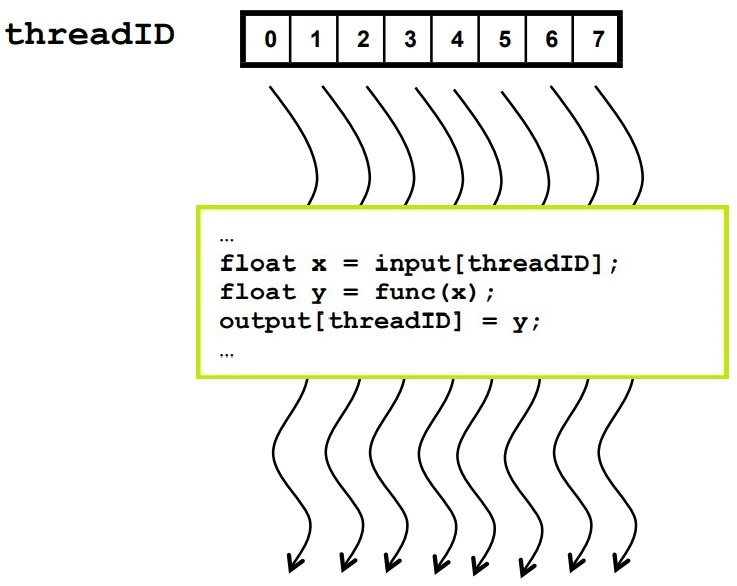
\includegraphics[width=9.5cm, keepaspectratio, clip]{images/ch01/CUDA_thread_parallelism.jpg}
	\caption{Execution of code by an 8-thread warp.
		The unique ID of each thread is stored in the variable \code{threadID}.
		In this example, \code{threadID} is used to read and write different data.
		Taken from \citetitle{Ruetsch2008} \cite{Ruetsch2008} and \citetitle{Cejka2022} \cite{Cejka2022}.
	}
	\label{Figure:theory->CUDA->thread-management->thread-parallelism}
\end{figure}

While threads in a warp execute in lockstep, they can diverge and execute different instructions.
This behavior is referred to as \textit{thread divergence} and it is discouraged as the execution will be serialized and thus suboptimal - see Figure~\ref{Figure:theory->CUDA->thread-management->thread-divergence} for a visualization of thread divergence.
Interestingly, until Nvidia's Volta generation was introduced in December 2017, thread divergence could lead to a deadlock in specific cases where sharing data between threads of a warp was required \cite{NVIDIADecember2022, Grote2020}.

\begin{figure}[ht!]
	\centering
	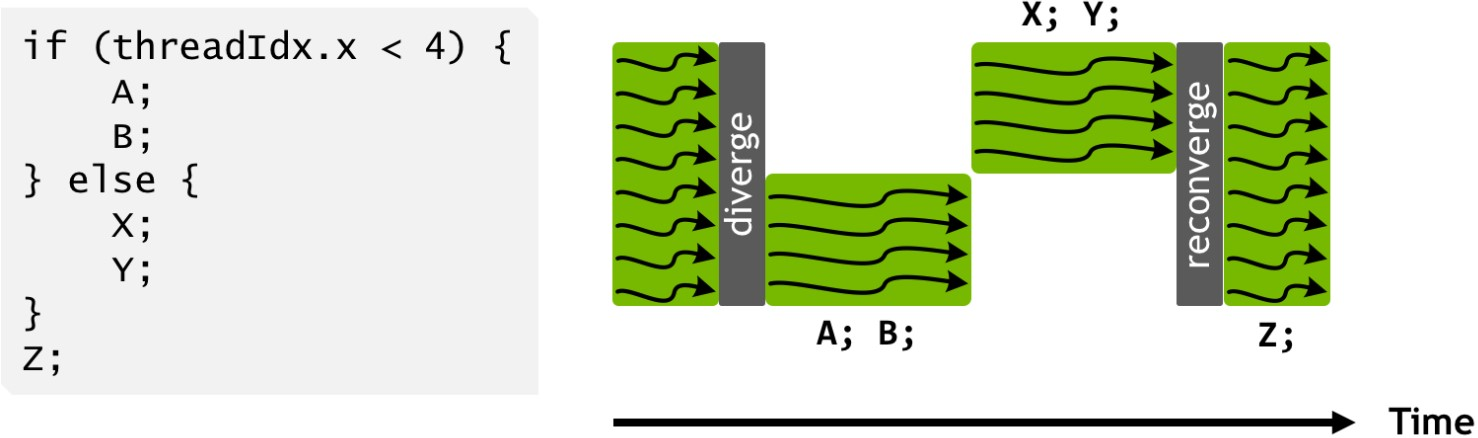
\includegraphics[width=14cm, keepaspectratio]{images/ch01/CUDA_warp_divergence_execution_path.jpg}
	\caption{Pseudocode showcasing thread divergence in an 8-thread warp.
		The \code{threadIdx.x} variable contains each thread's ID in the 1st dimension.
		In this example, while threads \code{0} to \code{3} execute statements \code{A} and \code{B}, threads \code{4} to \code{7} are idle.
		Then, threads \code{4} to \code{7} execute statements \code{X} and \code{Y} while threads \code{0} to \code{3} are idle.
		Finally, all threads resume lockstep execution with statement \code{Z}.
		Taken from Nvidia's developer blog post: \citetitle{Durant10May2017} \cite{Durant10May2017}.
	}
	\label{Figure:theory->CUDA->thread-management->thread-divergence}
\end{figure}

While CUDA provides special functions for intra-warp thread management \cite{Grover15January2018}, their use is not common compared to the use of thread groups higher in the hierarchy, called \textit{blocks}.

\paragraph{Block} To execute a group of threads they must first be grouped into a \textit{block}.
A single block can comprise up to 1024 threads (as of CUDA compute capability 3.5) that are organized in either 1D, 2D, or 3D \cite{NVIDIADecember2022}.
Every thread of a particular block has a unique ID per dimension, i.e., \code{x} for 1D, \code{x}, \code{y} for 2D, and \code{x}, \code{y}, \code{z} for 3D.
Combined with the fact that the threads of a warp are consecutive, choosing the dimension and size of a thread block can play a crucial role in achieving optimal performance.
To illustrate this, an example showing threads of a block divided into warps can be seen in Figure~\ref{Figure:theory->CUDA->thread-management->grouping-threads-in-block-into-warps}.

\begin{figure}[ht!]
	\centering
	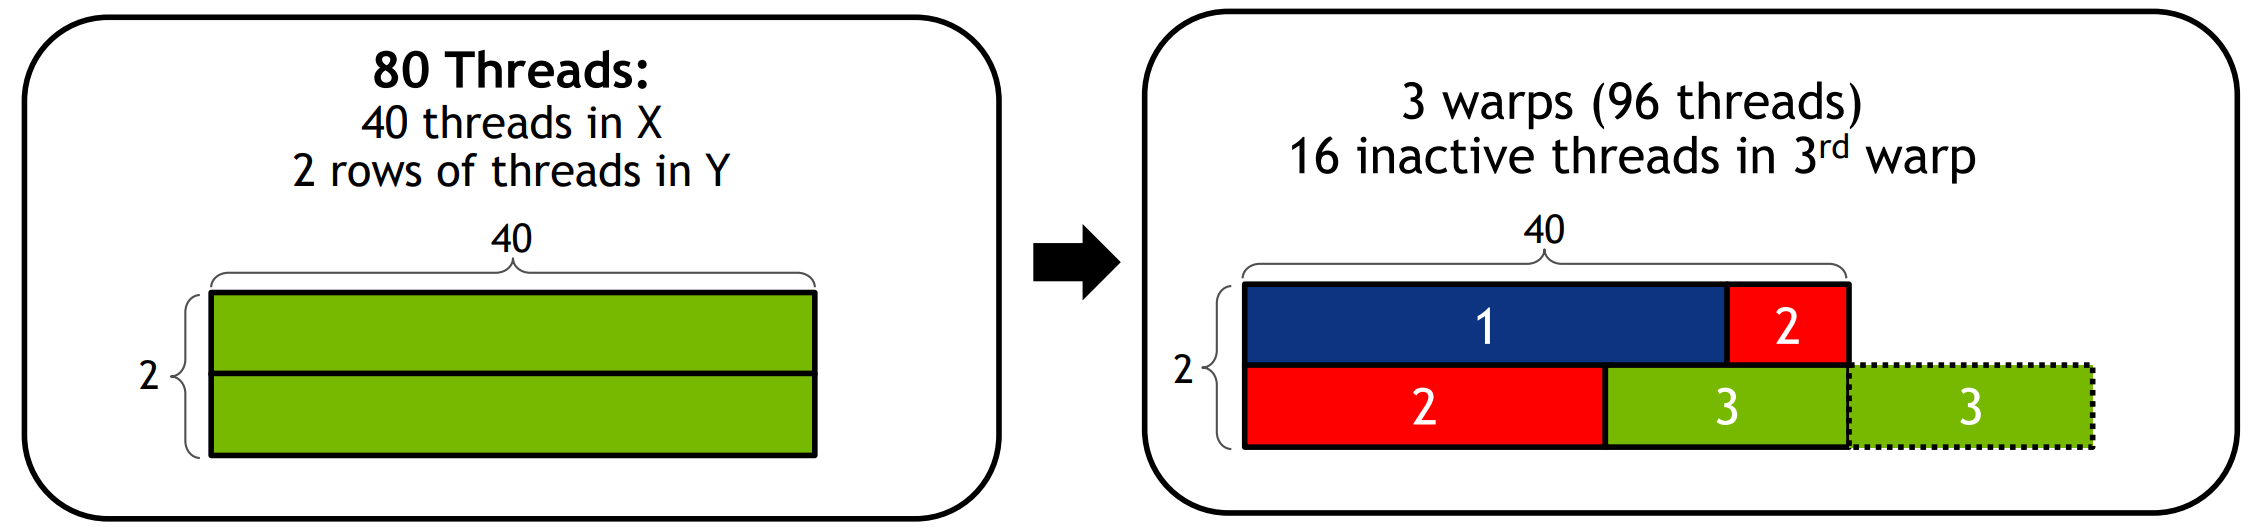
\includegraphics[width=\textwidth, keepaspectratio]{images/ch01/CUDA_threads_in_warp_and_block.png}
	\caption{Division of threads into warps in a block of 40 by 2 threads.
		Each green rectangle in the left image represents a row of threads.
		In the right image, each color represents a unique warp.
		Taken from \citetitle{ThomasCollignon2018} \cite{ThomasCollignon2018}.
	}
	\label{Figure:theory->CUDA->thread-management->grouping-threads-in-block-into-warps}
\end{figure}

As can be seen in Figure~\ref{Figure:theory->CUDA->thread-management->grouping-threads-in-block-into-warps}, since threads are consecutive in their 1st dimension, the 1st row of the block comprises 32 threads that belong to warp \code{0} (blue rectangle) and 8 threads from warp \code{1} (upper-right red square).
The 2nd row comprises 24 threads belonging to warp \code{1} (lower-right red rectangle) and 16 threads from warp \code{2} (left-most green rectangle).
While a warp can only consist of 32 consecutive threads, in warp \code{2}, only 16 will be utilized for execution, while the remaining 16 will remain inactive.

\paragraph{Grid} The final group of threads in the hierarchy, the \textit{grid}, comprises thread blocks.
Similarly to how threads are structured within a thread block, blocks can be structured within grids.
Grids can consist of up to 3 dimensions of blocks; each block has a unique ID per dimension.
Additionally, the limit of thread blocks per grid is bound to each dimension: the maximum number of blocks per dimension is 65,536.
For a visualization of a 2D grid comprising 2D thread blocks see Figure~\ref{Figure:theory->CUDA->thread-management->thread-management-system-overview}.

\begin{figure}[ht!]
	\centering
	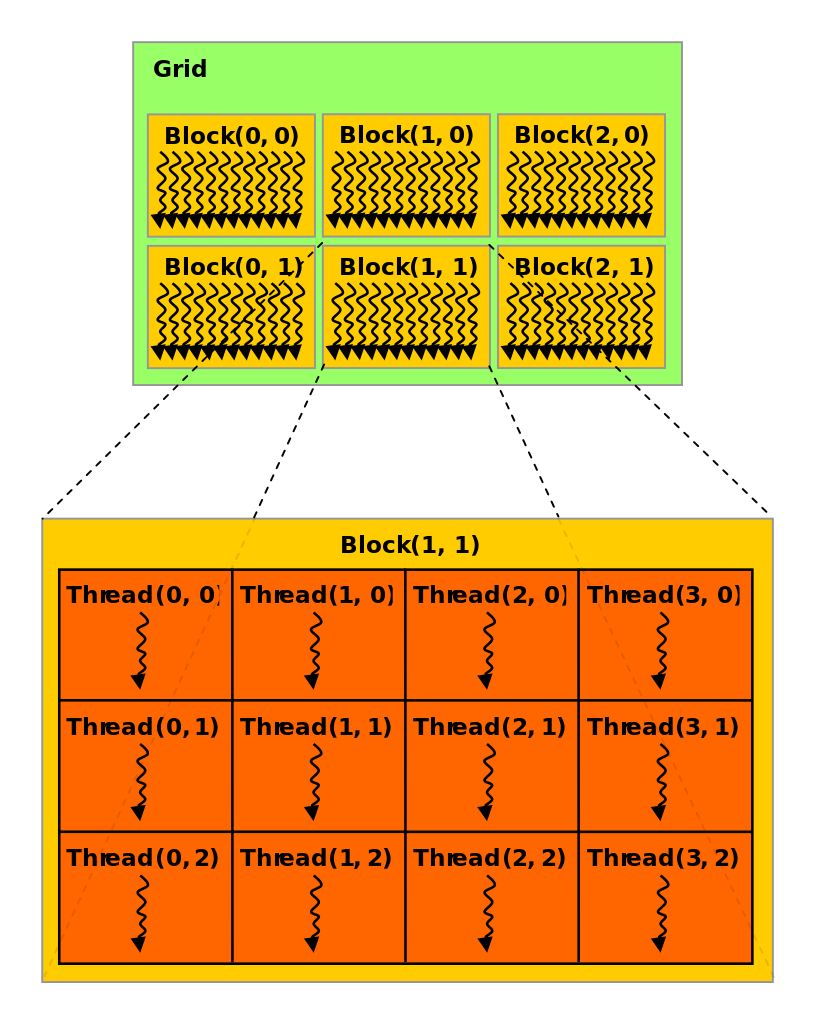
\includegraphics[width=12cm, keepaspectratio]{images/ch01/CUDA_thread_management_system_overview.png}
	\caption{Visualization of a 2-by-3 grid comprising 3-by-4 thread blocks.
		The numbers in the brackets are the IDs of each entity in each dimension.
		Taken from \citetitle{NVIDIADecember2022} \cite{NVIDIADecember2022}.
	}
	\label{Figure:theory->CUDA->thread-management->thread-management-system-overview}
\end{figure}

As shown in Figures \ref{Figure:theory->CUDA->thread-management->thread-parallelism} and \ref{Figure:theory->CUDA->thread-management->thread-divergence}, within a kernel, each thread has access to a collection of predefined variables unique to it.
The following is a selection of such commonly-used variables:

\begin{itemize}
	\item \code{threadIdx} - A 3-component vector containing the IDs of a thread in each dimension of a thread block.
Specifically, \code{threadIdx.x} contains the thread's ID in the 1st dimension (\code{x}), \code{threadIdx.y} in the 2nd dimension (\code{y}), and \code{threadIdx.z} in the 3rd dimension (\code{z}).
For example, in the 3-by-4 thread block shown in Figure~\ref{Figure:theory->CUDA->thread-management->thread-management-system-overview}, the values of \code{threadIdx} for the bottom-right-most thread are \code{\{3, 2, 1\}}, i.e., \code{threadIdx.x = 3}, \code{threadIdx.x = 2}, \code{threadIdx.z = 1}.
	\item \code{blockIdx} - A 3-component vector containing the IDs of a block in each dimension of a grid.
Similarly to \code{threadIdx}, each vector component contains the block's ID in a specific dimension, i.e., \code{blockIdx.x} contains the ID of the block in the 1st dimension (\code{x}), etc.
For example, for the bottom-right-most thread block shown in Figure~\ref{Figure:theory->CUDA->thread-management->thread-management-system-overview}, \code{blockIdx} would be \code{\{2, 1, 1\}}, i.e., \code{blockIdx.x = 2}, \code{blockIdx.y = 1}, \code{blockIdx.z = 1}.
	\item \code{blockDim} - A 3-component vector containing the sizes of a block's dimensions.
For example, for the thread block shown in Figure~\ref{Figure:theory->CUDA->thread-management->thread-management-system-overview}, \code{blockDim} would be \code{\{3, 4, 1\}}, i.e., \code{blockDim.x = 3}, \code{blockDim.y = 4}, \code{blockDim.z = 1}.
\end{itemize}

For a summarized overview of predefined variables and functions available, see \citetitle{Gates2023} \cite{Gates2023} or see \citetitle{NVIDIADecember2022} \cite{NVIDIADecember2022} for an extensive overview.

The variables listed earlier are often used to compute the global ID of a thread in a dimension of a grid:
$$\code{globalID = blockIdx.x * blockDim.x + threadIdx.x}$$

In a standard setup, the grid is the upper-most thread grouping in CUDA's thread management hierarchy.
As visualized in Figure~\ref{Figure:theory->CUDA->thread-management->thread-structures-executed-by-hardware}, when a kernel is executed on the device, it is executed on all threads of a grid.

\begin{figure}[ht!]
	\centering
	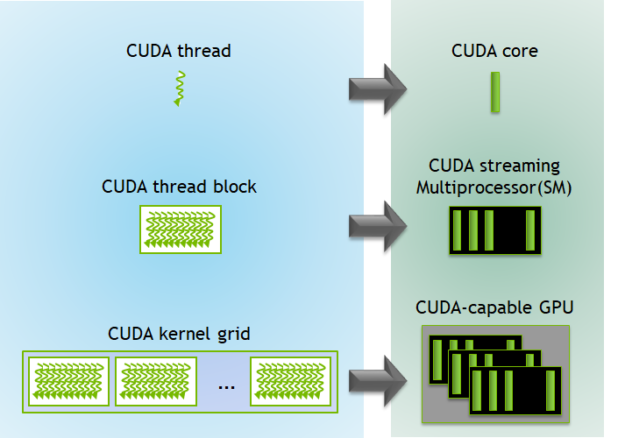
\includegraphics[width=12cm, keepaspectratio]{images/ch01/CUDA_structures_executed_by_hardware.png}
	\caption{Visualization illustrating the execution of CUDA thread structures by different hardware components in an Nvidia GPU.
		Taken from \citetitle{Gupta26June2020} \cite{Gupta26June2020}.
	}
	\label{Figure:theory->CUDA->thread-management->thread-structures-executed-by-hardware}
\end{figure}

To execute a kernel on the device, it is necessary to provide the kernel with an execution configuration: \code{$<$$<$$<$ Dg, Db, Ns, S $>$$>$$>$}, where:
\begin{itemize}
	\item \code{Dg} - dimension and size of the grid;
	\item \code{Db} - dimension and size of each block;
	\item \code{Ns} - optional (default value is 0), number of bytes in shared memory allocated per block in addition to statically allocated shared memory (explained in Section~\ref{Subsection:theory->CUDA->memory-management});
	\item \code{S} - optional (default value is 0), stream associated with the kernel (explained in Section~\ref{Subsection:theory->CUDA->concurrent-kernel-execution}).
\end{itemize}

An example of a kernel call with a basic execution configuration is presented in Listing~\ref{Listing:theory->CUDA->thread-management->kernel-configuration-example}.

\begin{lstlisting}[caption={Excerpt of C++ code portraying the creation of a grid configuration and the launching of a kernel.
The example implementation aims to increment every value of the \code{N}-by-\code{N} matrix \code{mtx} by 1 using the device. \code{dim3} is an integer vector type based on \code{uint3} that is used to specify dimensions - unspecified components are implicitly set to 1 \cite{NVIDIADecember2022}.
Taken from \citetitle{NVIDIADecember2022} \cite{NVIDIADecember2022}.},label={Listing:theory->CUDA->thread-management->kernel-configuration-example}]
// Kernel definition
__global__ void AddOneToMatrix( float mtx[N][N] )
{
	// Get thread ID for each dimension to use as matrix indices
	int row = blockIdx.x * blockDim.x + threadIdx.x;
	int col = blockIdx.y * blockDim.y + threadIdx.y;
	
	// Check if the indices are within the dimensions of the matrix
	if( row < N && col < N ) {
		mtx[row][col] += 1;
	}
}

int main()
{
	...
	// Number of threads in each 2D block is 16x16 = 256
	dim3 threadsPerBlock( 16, 16 );
	
	// Number of blocks in the grid depends on the matrix dimension (NxN)
	dim3 numBlocks( N / threadsPerBlock.x, N / threadsPerBlock.y );
	
	// Kernel that computes: mtx = mtx + 1 (element-wise)
	AddOneToMatrix<<< numBlocks, threadsPerBlock >>>( mtx );
	...
}
\end{lstlisting}

In Listing~\ref{Listing:theory->CUDA->thread-management->kernel-configuration-example}, the code in the \code{main()} function is executed on the host while the code in the \code{AddOneToMatrix(...)} kernel is executed on the device.
From the host's point of view, kernel calls are asynchronous.
In other words, the host will call for the kernel to be executed on the device and then it will move on to the next line of execution without delay.
This holds even if the host calls two kernels in succession.
In such a case, from the device's point of view, the two kernels will be executed in the order they were called.

\subsection{Memory Management}\label{Subsection:theory->CUDA->memory-management}
This section will briefly introduce the memory management system present in CUDA - for a comprehensive overview see \citetitle{Cejka2020} \cite{Cejka2020} and \citetitle{Cejka2022} \cite{Cejka2022}.

Similarly to the layout in Section~\ref{Subsection:theory->CUDA->thread-management}, the memory management system of CUDA will be briefly described starting with the most fundamental type of memory and advancing to the highest level.

\paragraph{Registers and Local Memory} While executing a kernel, each thread has access to a memory space that is unique to it, i.e., other threads cannot access it.
The lifetime of this memory is bound to the context of the kernel it is allocated with.
This space encompasses two separate memories: \textit{registers} and \textit{local memory}.

\textit{Registers} are fast 32-bit on-chip memories (low latency and high bandwidth) that are often used for storing variables unique to each thread.
The number of registers available to a thread in the context of a kernel is limited to 255 (since CUDA compute capability 3.2) \cite{NVIDIADecember2022}.
If a variable or structure allocated in the context of a kernel exceeds the registers available to a thread, then the compiler stores them in \textit{local memory} - this behavior is referred to as \textit{register spilling}.

\textit{Local memory} resides in off-chip device memory (referred to as \textit{global memory}; high latency and low bandwidth) which is slower to access than registers.
Local memory for each thread is limited to 512 KB \cite{NVIDIADecember2022}.

While using registers to store frequently-accessed indexing variables can help improve performance, it should be done with care to avoid the performance loss associated with register spilling.

\paragraph{Shared Memory} In the context of a kernel, all threads of a block have access to a block-unique memory space referred to as \textit{shared memory}.
Similarly to \textit{registers}, shared memory is located on-chip and is therefore high-speed.
The maximum size of shared memory per block varies depending on the CUDA compute capability version as shown in Table ~\ref{Table:theory->CUDA->memory-management->max-shared-memory-per-block-based-on-compute-capability}.

\begin{table}[ht!]
	\centering
	\begin{tabular}{|c|c|c|c|c|c|c|c|}
		\hline
		\cellcolor[HTML]{C0C0C0}\textbf{Compute capability}                & 7.0 - 7.2 & 7.5 & 8.0 & 8.6 & 8.7 & 8.9 & 9.0 \\ \hline
		\cellcolor[HTML]{C0C0C0}\textbf{Max. shared memory per block [KB]} &    96     & 64  & 163 & 99  & 163 & 99  & 227 \\ \hline
	\end{tabular}
	\caption{Maximum shared memory per thread block depending on the CUDA compute capability version.
		Note that to use more than 48 KB, dynamic shared memory must be used.
		Taken from \citetitle{NVIDIADecember2022} \cite{NVIDIADecember2022}.
	}
	\label{Table:theory->CUDA->memory-management->max-shared-memory-per-block-based-on-compute-capability}
\end{table}

Shared memory can be allocated statically, dynamically, or both.
The amount of statically allocated memory is known at compile time while the amount of dynamically allocated memory is known at run time \cite{Harris28January2013}.
Note that the total amount of shared memory allocated for a thread block is equal to the sum of statically and dynamically allocated shared memory.

Since \textit{statically} allocated shared memory is known at compile time, it must be declared with a size known at compile time.
It is often declared inside a kernel using the \code{\_\_shared\_\_} modifier.

On the other hand, the size of \textit{dynamically} allocated memory must be supplied as one of the kernel launch parameters as mentioned in Section~\ref{Subsection:theory->CUDA->thread-management}.

Listing~\ref{Listing:theory->CUDA->memory-management->statically-allocated-shared-memory-example} shows an excerpt of C++ code where the syntax for static and dynamic memory allocation is presented - for the full code see \citetitle{Harris28January2013} by \citename{Harris28January2013}{author} \cite{Harris28January2013}.

\begin{lstlisting}[caption={Excerpt of C++ code showcasing the syntax of static and dynamic shared memory allocation.
Note when an array in shared memory is declared using \code{extern}, then the size of the array is determined at run time \cite{NVIDIADecember2022}.
Taken from \citetitle{Harris28January2013} by \citename{Harris28January2013}{author} \cite{Harris28January2013}.},label={Listing:theory->CUDA->memory-management->statically-allocated-shared-memory-example}]
__global__ void kernel( ... )
{
	...
	// Declare statically allocated shared memory
	__shared__ int s_s[32];

	// Access dynamically allocated shared memory
	extern __shared__ int s_d[];
	...
}

int main()
{
	...
	const int n = 64;
	
	// Launch kernel with:
	// - 32*sizeof(int) bytes of statically allocated shared memory
	// - n*sizeof(int) bytes of dynamically allocated shared memory
	kernel<<< 1, n, n*sizeof(int) >>>( ... );
	...
}
\end{lstlisting}

For more information regarding shared memory see Section~1.2.3 in \citetitle{Cejka2022} \cite{Cejka2022} or \citetitle{NVIDIADecember2022} \cite{NVIDIADecember2022}.

\paragraph{Global Memory} The largest memory space present in CUDA is \textit{global memory}.
It is occasionally referred to as \textit{device memory} as it resides in an Nvidia GPU's DRAM (Dynamic Random Access Memory).
While global memory resides in a device's memory, it can be accessed by both the host and the device, thus creating a communication medium between the two.
The amount of global memory available depends on the GPU used, for example, the Nvidia A100 GPU is available with either 40 GB or 80 GB (shown in Table~\ref{Table:theory->GPUs->GPGPU->nvidia-gpu-details-comparison}).
Although it is the largest memory space found on the device, it is high-latency and low-bandwidth compared to, e.g., shared memory.

To clarify, since global memory is accessible by the device, it can be accessed by any thread of any grid.
See Figure~\ref{Figure:theory->CUDA->memory-management->memory-spaces} for a visualization of CUDA thread structures and the memory spaces accessible to them.

\begin{figure}[ht!]
	\centering
	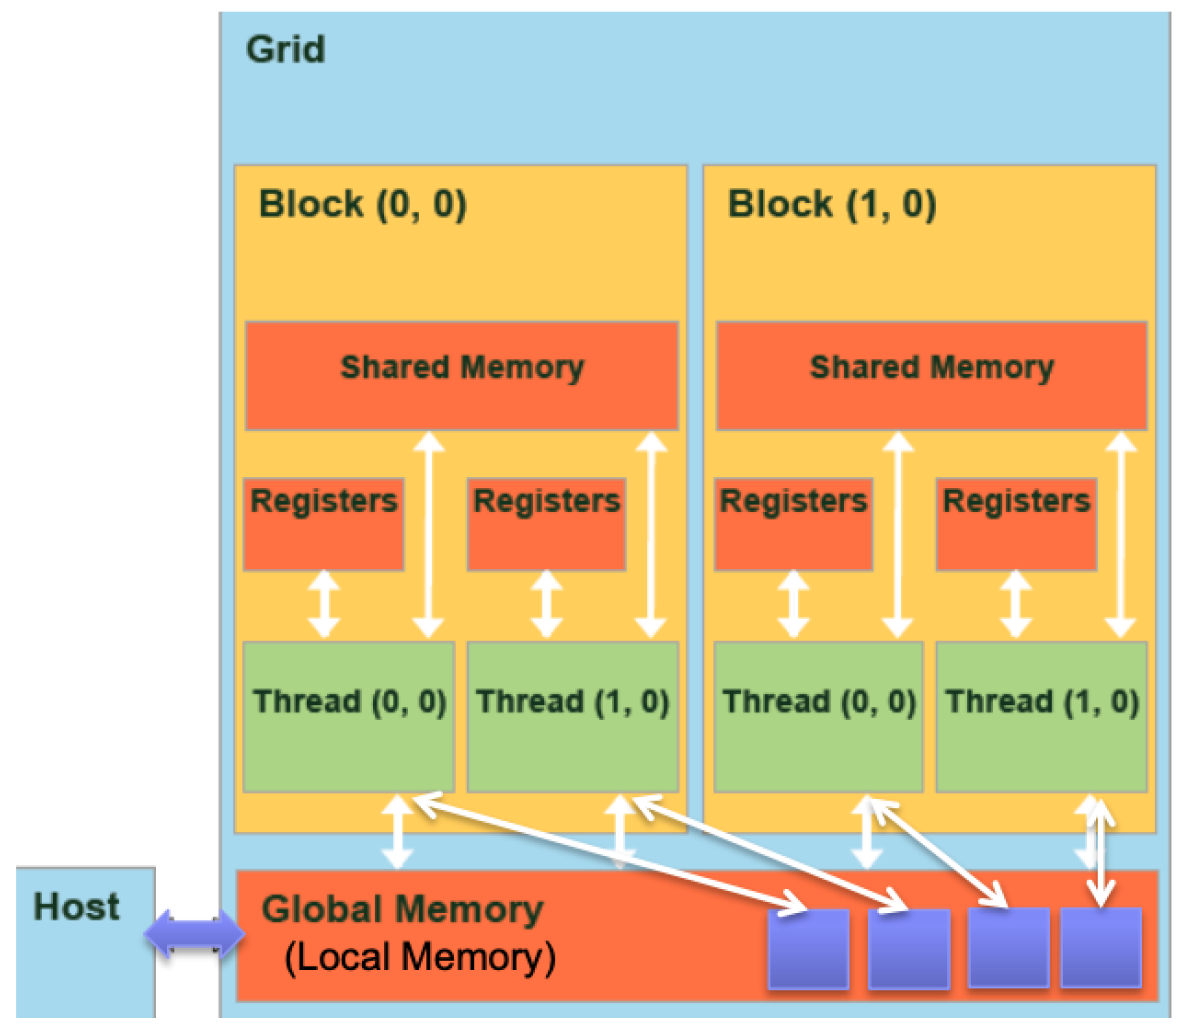
\includegraphics[width=12cm, keepaspectratio]{images/ch01/CUDA_memory_types_detailed.png}
	\caption{CUDA memory structuring with accesses available to each thread structure.
		Taken from \citetitle{Hsiao17December2019} by \citename{Hsiao17December2019}{author} \cite{Hsiao17December2019}.
	}
	\label{Figure:theory->CUDA->memory-management->memory-spaces}
\end{figure}

Furthermore, unlike the aforementioned memory spaces, the lifetime of global memory is bound to the CUDA application, i.e., data can be present in global memory when the application starts and removed when the application terminates.
Moreover, global memory requires explicit allocation, copying, and deallocation of data - see \citetitle{Cejka2022} \cite{Cejka2022} and \citetitle{NVIDIADecember2022} \cite{NVIDIADecember2022} for the specific functions.

For completeness, Figure~\ref{Figure:theory->CUDA->memory-management->nvidia-gpu-architecture-and-cuda-structures} shows the architecture of an Nvidia GPU along with an overview of the CUDA programming model.

\begin{figure}[ht!]
	\centering
	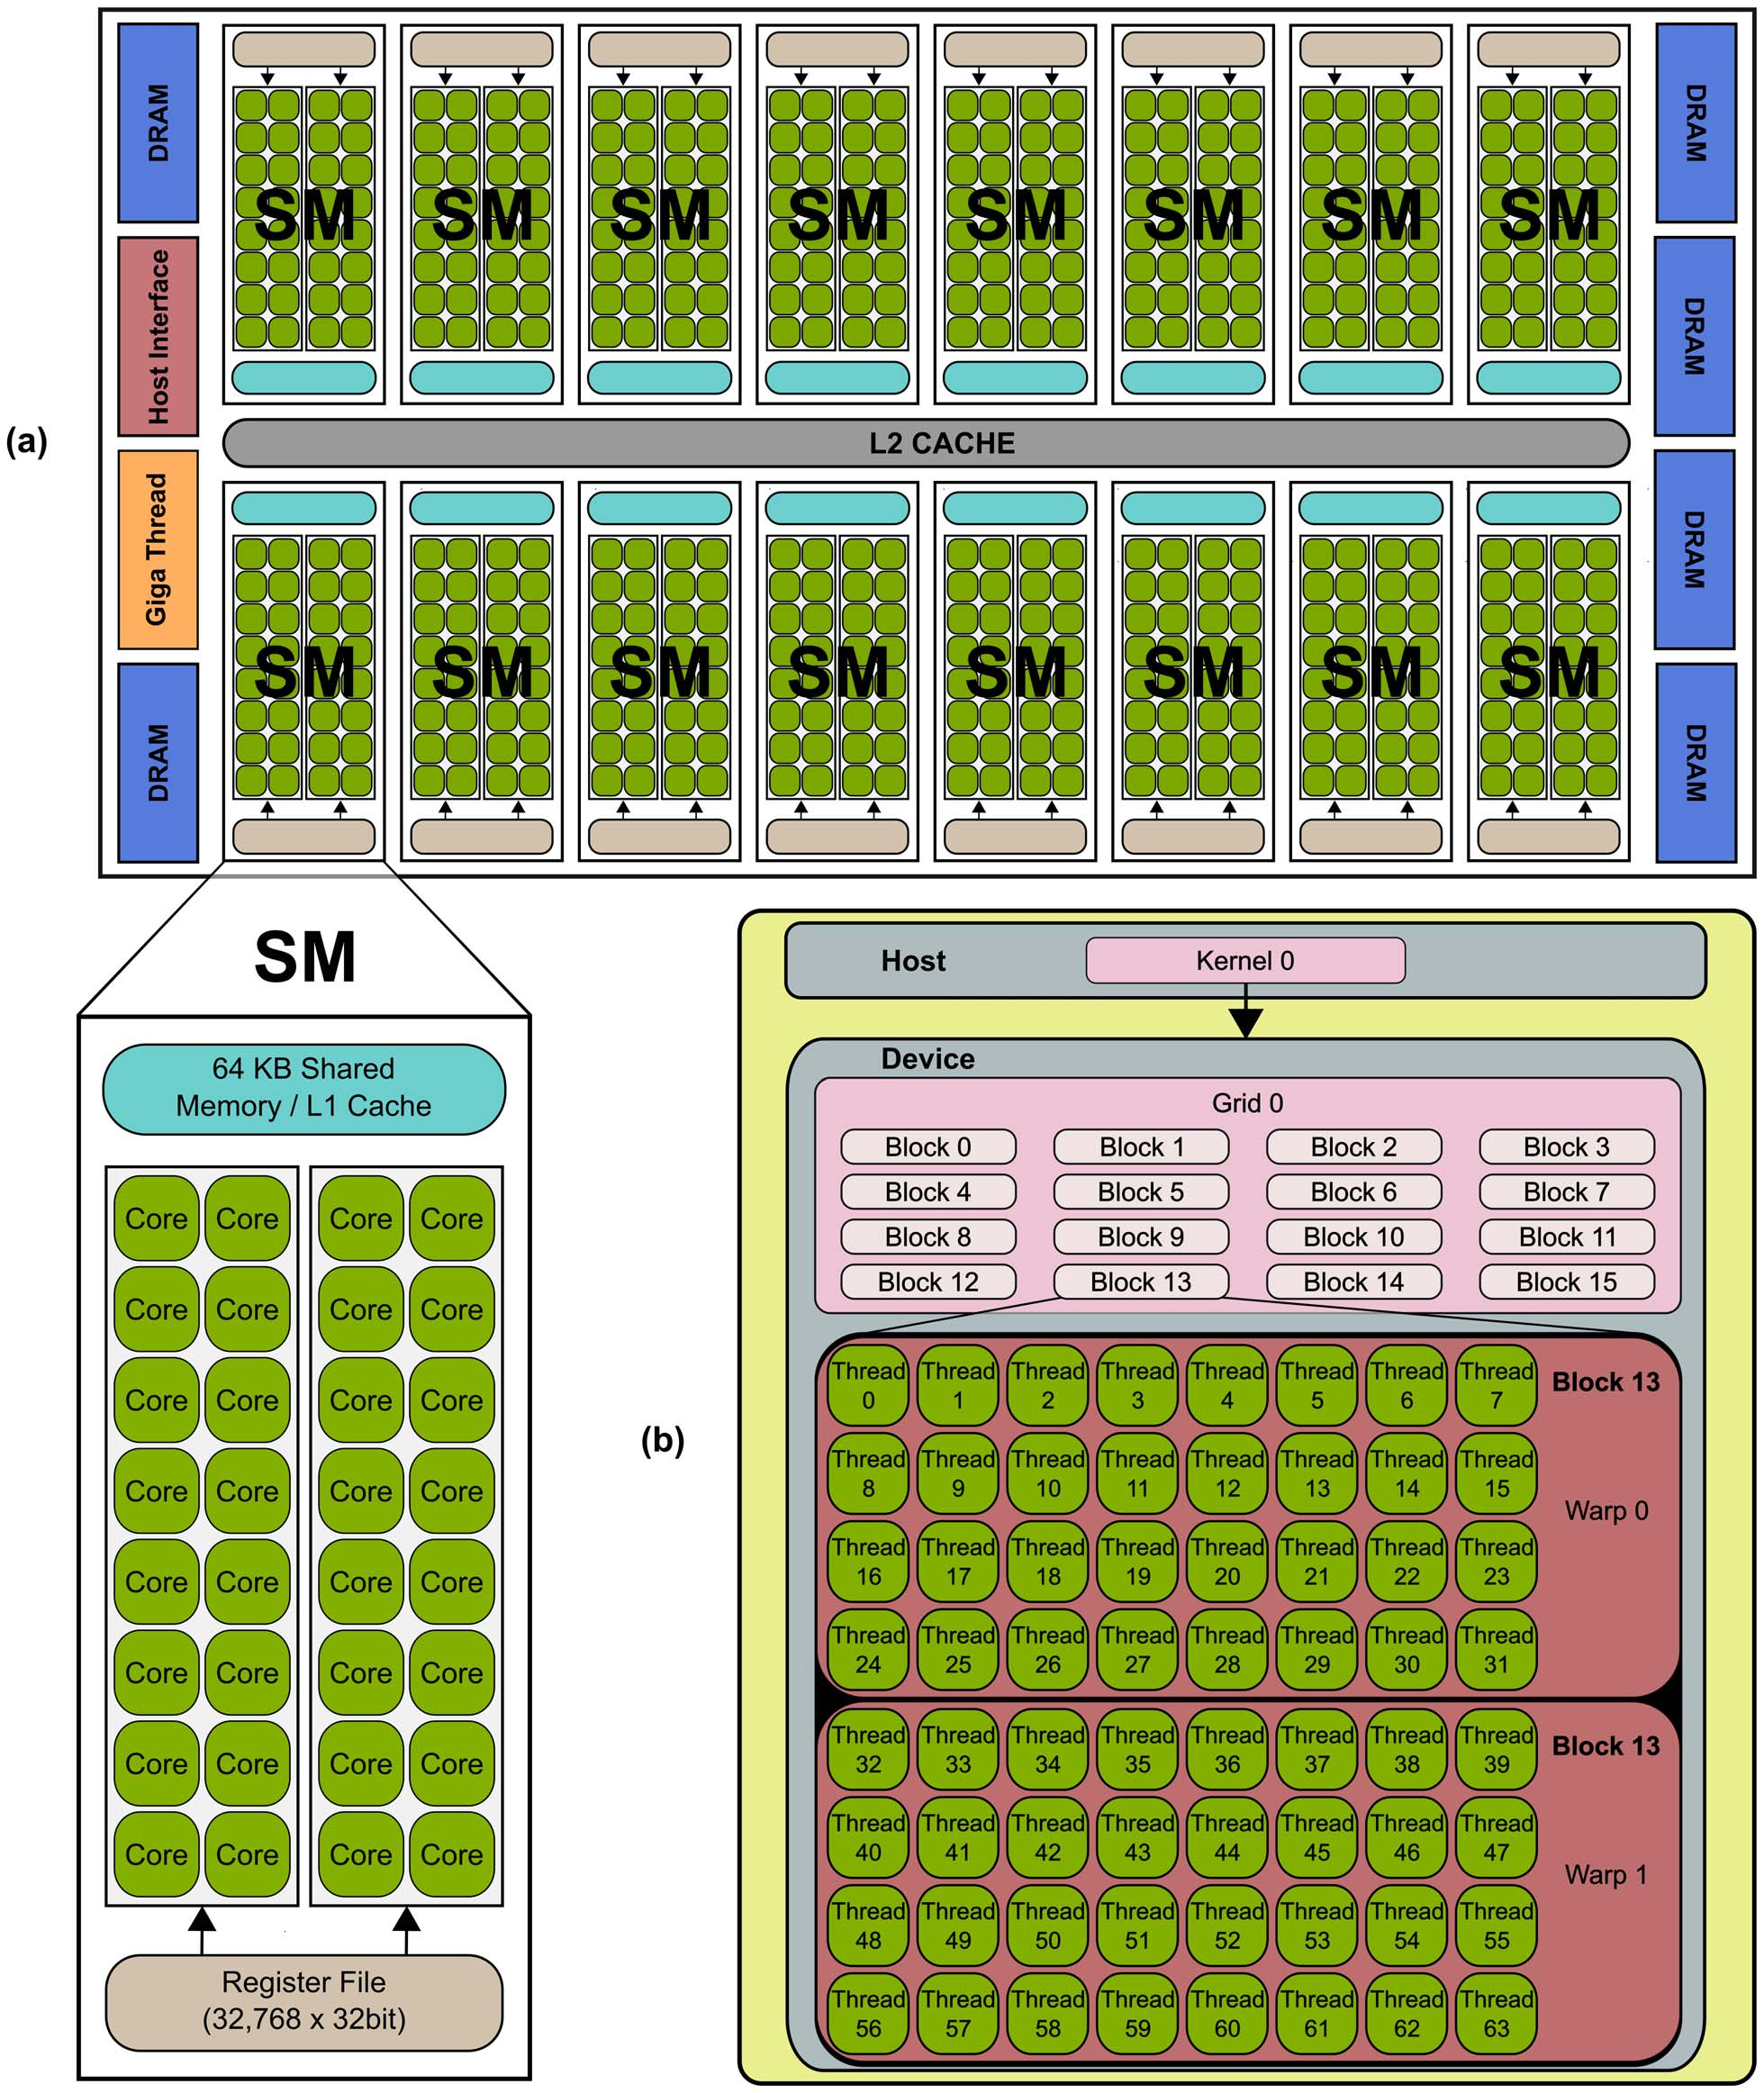
\includegraphics[width=\textwidth, keepaspectratio]{images/ch01/nvidia_gpu_architecture_and_cuda_structures.png}
	\caption{Simplified overview of an Nvidia GPU's architecture and the CUDA programming model.
		Taken from \citetitle{Hernandez2015} \cite{Hernandez2015}.
	}
	\label{Figure:theory->CUDA->memory-management->nvidia-gpu-architecture-and-cuda-structures}
\end{figure}

While there is only one kernel present in Figure~\ref{Figure:theory->CUDA->memory-management->nvidia-gpu-architecture-and-cuda-structures}, it is noteworthy that if another kernel was launched concurrently (explained later in Section~\ref{Subsection:theory->CUDA->concurrent-kernel-execution}) the threads allocated to it would also have access to global memory.
In other words, global memory is the same for all kernels in a CUDA application.

\subsection{Concurrent Kernel Execution}\label{Subsection:theory->CUDA->concurrent-kernel-execution}
Concurrent kernel execution describes a scenario where two or more kernels from the same CUDA application are running simultaneously.
Note that kernels can be executed concurrently only on certain devices with compute capability 2.x or higher.
To check whether a device is capable of concurrent kernel execution, the \code{deviceQuery} executable provided with the CUDA Toolkit can be used \cite{NVIDIADecember2022}.

\paragraph{Streams} As mentioned in Section~\ref{Subsection:theory->CUDA->thread-management}, tasks on the device are executed serially, i.e., in the order the host launched them.
This series of tasks is referred to as the \textit{default stream} since it is present implicitly.
To execute kernels concurrently, it is necessary to use multiple \textit{streams}.
Nvidia defines a stream as "\textit{a sequence of commands that execute in order}" \cite{NVIDIADecember2022}.

Additionally, in Section~\ref{Subsection:theory->CUDA->thread-management}, it was mentioned that a kernel is launched on a grid made up of thread blocks.
This holds even when multiple kernels are launched simultaneously, i.e., each kernel is launched on a separate grid.
When a grid is executing a kernel it is referred to as a resident grid.

Note that the use of concurrent kernel execution is associated with certain limitations \cite{Cejka2022, NVIDIADecember2022}:

\begin{enumerate}
	\item Maximum number of resident grids per device.
	\item Kernels from different CUDA contexts cannot be run concurrently.
	\item Kernels are only run concurrently if the device has enough resources for them.
	\item Undefined behavior during stream interaction.
\end{enumerate}

The first limitation is dependent on the compute capability version as presented in Table~\ref{Table:theory->CUDA->concurrent-kernel-execution->maximum-resident-grids-per-device}.

\begin{table}[ht!]
	\centering
	\begin{tabular}{|c|c|c|c|}
		\hline
		\cellcolor[HTML]{C0C0C0}\textbf{Compute capability}             & 7.0 & 7.2 & 7.5 - 9.0 \\ \hline
		\cellcolor[HTML]{C0C0C0}\textbf{Max. resident grids per device} & 128 & 16  &    128    \\ \hline
	\end{tabular}
	\caption{Maximum number of resident grids on one device for CUDA compute capability 7.0 and higher.
		Taken from \citetitle{NVIDIADecember2022} \cite{NVIDIADecember2022}.
	}
	\label{Table:theory->CUDA->concurrent-kernel-execution->maximum-resident-grids-per-device}
\end{table}

The second limitation prevents the concurrent execution of kernels from two distinct CUDA applications on the same device.
In particular, if kernels are issued from distinct processes, they cannot run concurrently unless CUDA MPS\footnote{CUDA MPS documentation website URL: \url{https://docs.nvidia.com/deploy/mps/index.html}} is used \cite{Crovella16December2016, Crovella17August2017}.

The third limitation states that a device can only run kernels concurrently if its resource limits are not overstepped.
However, this does not mean that the kernels will not be run.
On the contrary, if two or more kernels are launched using unique streams and the device's resources cannot satisfy the sum of resources required by the kernels, then one of the kernels will be executed first while the other kernels are put aside until resources are available for them.
In this context, resources are either local memory or the number of threads the device is capable of running at a point in time.

The fourth limitation is often issued as a disclaimer from Nvidia that warns against the interactivity of streams.
Specifically, since all streams are independent of each other and have access to the same global memory, one stream can alter the data used by another stream resulting in inconsistent and possibly erroneous behavior.

To prevent the unpredictable execution order of stream-unique kernels, explicit synchronization can be used.
Functions providing explicit synchronization are, for example:

\begin{itemize}
	\item \code{cudaDeviceSynchronize()} - This function creates a checkpoint where the host waits until all preceding commands in all streams of all host threads have been completed \cite{NVIDIADecember2022}.
	\item \code{cudaStreamSynchronize( stream )} - This function serves a similar purpose to \code{cudaDeviceSynchronize()} with the exception that the host only waits until the preceding commands of a specific stream have completed.
\end{itemize}

To use a stream, other than the default stream, it is first necessary to construct it by instantiating and creating a stream object using \code{cudaStream\_t} and \code{cudaStreamCreate()}.
Then, the stream must be supplied to a kernel's execution configuration to launch the kernel using it.
Once the stream is no longer needed it must be destroyed using \code{cudaStreamDestroy()}.
C++ pseudocode detailing the creation, usage, and destruction of streams is shown in Listing~\ref{Listing:theory->CUDA->concurrent-kernel-execution->creation-usage-destruction-of-streams}.

\begin{lstlisting}[caption={C++ pseudocode showcasing the creation, usage, and destruction of two streams.
Taken from \citetitle{NVIDIADecember2022} \cite{NVIDIADecember2022}.},label={Listing:theory->CUDA->concurrent-kernel-execution->creation-usage-destruction-of-streams}]
	// Declare array of 2 stream objects
	cudaStream_t streams[ 2 ];
	
	// Create each stream
	for( int i = 0; i < 2; ++i ) {
		cudaStreamCreate( &streams[ i ] );
	}
	
	// Launch MyKernelA using the 0th stream on a grid of one one-thread block with 0 bytes of dynamically allocated shared memory
	MyKernelA<<< 1, 1, 0, stream[ 0 ] >>>( inputVariableA )
	
	// Launch MyKernelB using the 1st stream
	MyKernelB<<< 1, 1, 0, stream[ 1 ] >>>( inputVariableB )
	
	// Destroy each stream
	for( int i = 0; i < 2; ++i ) {
		cudaStreamDestroy( stream[ i ] );
	}
\end{lstlisting}

Assuming that the total local memory required by both kernels called in Listing~\ref{Listing:theory->CUDA->concurrent-kernel-execution->creation-usage-destruction-of-streams} can be provided by a device at a point in time, they will be executed in parallel.
For a visualization of concurrent kernel execution see Figure~\ref{Figure:theory->CUDA->concurrent-kernel-execution->concurrent-kernel-execution-visualization}.

\begin{figure}[ht!]
	\centering
	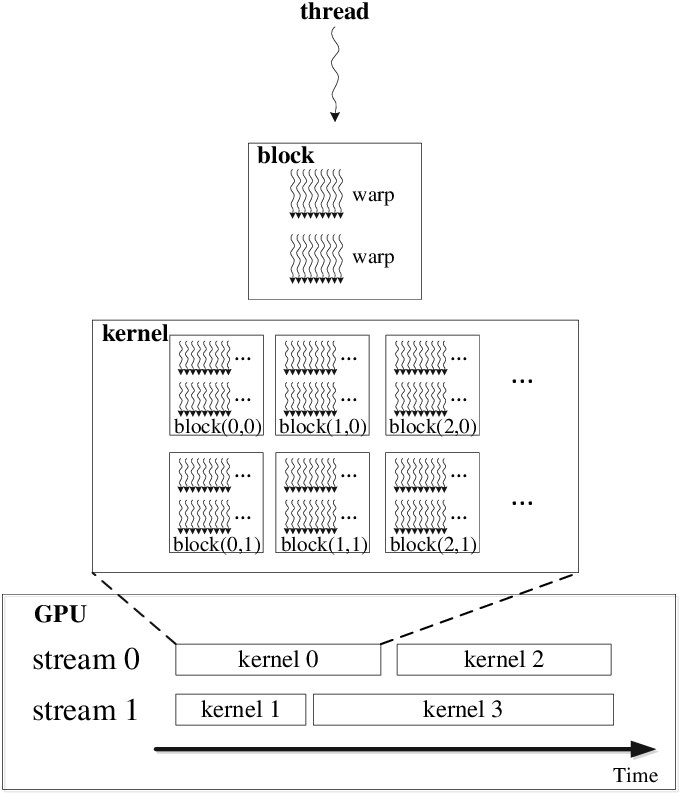
\includegraphics[width=11cm, keepaspectratio]{images/ch01/CUDA_concurrent_kernel_execution.png}
	\caption{Visualization of concurrent kernel execution.
		Taken from \citetitle{Xu2015} \cite{Xu2015}.
	}
	\label{Figure:theory->CUDA->concurrent-kernel-execution->concurrent-kernel-execution-visualization}
\end{figure}

\subsection{Parallel Reduction}\label{Subsection:theory->CUDA->parallel-reduction}
This section aims to present a parallel computation concept relevant to the project.
As stated earlier in Section~\ref{Subsection:theory->GPUs->GPGPU}, the parallelization of certain tasks is not straightforward.
An example of such a task is finding the maximum value in an array.

The naive procedure for finding the maximum value is to iterate through the array, compare each encountered element to a temporary variable, and save the larger of the two compared values into the variable.
However, this procedure is strictly sequential and thus inefficient when performed on the device in its current form.
In this case, \textit{parallel reduction} can be used to parallelize the problem.

Parallel reduction is a means of reducing the values of an array into a single value using an associative binary operator \cite{Kirk2013}.
The operators often used in parallel reduction are, for example, $\min$, $\max$, $\argmin$, $\argmax$, $\mathrm{sum}$, etc.
To clearly explain parallel reduction, the $\max$ operator will be assumed.

In the context of CUDA, finding the maximum value of an array stored in global memory is a two-step procedure:

\begin{enumerate}
	\item A kernel is launched in which each thread block copies a subarray into shared memory and finds its maximum value.
The block then saves the maximum value into another array stored in global memory.
This process is repeated for the array comprising of per-block maximum values until the number of elements required for comparison is smaller than the maximum number of threads a block can have.
	\item The kernel is launched again on a grid comprising a single thread block.
This allows loading the entire array into the block's shared memory, which means that the maximum value produced will be the largest in the initial array.
\end{enumerate}

To clearly explain parallel reduction, an example detailing the kernel will be described, i.e., finding the maximum value of an array stored in shared memory.

In short, parallel reduction performs iterations of simultaneous pair-comparisons as shown in Figure~\ref{Figure:theory->CUDA->parallel-reduction->maximum-value-in-array-using-parallel-reduction-with-interleaved-addressing}.

\begin{figure}[!ht]
	\centering
	\begin{tikzpicture}[scale=0.75]
		\tikzstyle{box} = [draw, fill=gray!20, minimum size=0.8cm]
		\tikzstyle{thread} = [draw, circle, fill=nvidia-light, minimum size=0.64cm]
		
		% Iteration: 1
		%% Array
		\def\numElems{16}
		\pgfmathtruncatemacro{\lastIdx}{\numElems - 1}
		\foreach \idx in {0, ..., \lastIdx}{
			\node[box] at (\idx, 12) (iterOneArr\idx) {$\idx$};
		}
		%% Threads and arrows
		\pgfmathtruncatemacro{\iterOneLastThread}{\numElems/2 - 1}
		\foreach \tid in {0, ..., \iterOneLastThread}{
			\pgfmathtruncatemacro{\idxLeft}{2^1 * \tid}
			\pgfmathtruncatemacro{\idxRight}{\idxLeft + 2^0}
			\node[thread] at (\idxLeft, 10.5) (iterOneThread\tid) {$\tid$};
			\draw[-latex] (iterOneArr\idxLeft.south) to (iterOneThread\tid.north);
			\draw[-latex] (iterOneArr\idxRight.south) to [bend left] (iterOneThread\tid.east);
		}	
		
		% Iteration: 2
		%% Array
		\foreach \idx/\elem in {0/1, 1/1, 2/3, 3/3, 4/5, 5/5, 6/7, 7/7, 8/9, 9/9, 10/11, 11/11, 12/13, 13/13, 14/15, 15/15}{
			\node[box] at (\idx, 9) (iterTwoArr\idx) {$\elem$};
		}
		%% Arrows from above
		\foreach \tid in {0, ..., \iterOneLastThread}{
			\pgfmathtruncatemacro{\idx}{2^1 * \tid}
			\draw[-latex] (iterOneThread\tid) to (iterTwoArr\idx);
		}
		%% Threads and arrows
		\pgfmathtruncatemacro{\iterTwoLastThread}{\numElems/2/2 - 1}
		\foreach \tid in {0, ..., \iterTwoLastThread}{
			\pgfmathtruncatemacro{\idxLeft}{2^2 * \tid}
			\pgfmathtruncatemacro{\idxRight}{\idxLeft + 2^1}
			\node[thread] at (\idxLeft, 7.5) (iterTwoThread\tid) {$\tid$};
			\draw[-latex] (iterTwoArr\idxLeft.south) to (iterTwoThread\tid.north);
			\draw[-latex] (iterTwoArr\idxRight.south) to [bend left] (iterTwoThread\tid.east);
		}
		
		% Iteration: 3
		%% Array
		\foreach \idx/\elem in {0/3, 1/1, 2/3, 3/3, 4/7, 5/5, 6/7, 7/7, 8/11, 9/9, 10/11, 11/11, 12/15, 13/13, 14/15, 15/15}{
			\node[box] at (\idx, 6) (iterThreeArr\idx) {$\elem$};
		}
		%% Arrows from above
		\foreach \tid in {0, ..., \iterTwoLastThread}{
			\pgfmathtruncatemacro{\idx}{2^2 * \tid}
			\draw[-latex] (iterTwoThread\tid) to (iterThreeArr\idx);
		}
		%% Threads and arrows
		\pgfmathtruncatemacro{\iterThreeLastThread}{\numElems/2/2/2 - 1}
		\foreach \tid in {0, ..., \iterThreeLastThread}{
			\pgfmathtruncatemacro{\idxLeft}{2^3 * \tid}
			\pgfmathtruncatemacro{\idxRight}{\idxLeft + 2^2}
			\node[thread] at (\idxLeft, 4.5) (iterThreeThread\tid) {$\tid$};
			\draw[-latex] (iterThreeArr\idxLeft.south) to (iterThreeThread\tid.north);
			\draw[-latex] (iterThreeArr\idxRight.south) to [bend left=15, in=170] (iterThreeThread\tid.east);
		}
		
		% Iteration: 4
		%% Array
		\foreach \idx/\elem in {0/7, 1/1, 2/3, 3/3, 4/7, 5/5, 6/7, 7/7, 8/15, 9/9, 10/11, 11/11, 12/15, 13/13, 14/15, 15/15}{
			\node[box] at (\idx, 3) (iterFourArr\idx) {$\elem$};
		}
		%% Arrows from above
		\foreach \tid in {0, ..., \iterThreeLastThread}{
			\pgfmathtruncatemacro{\idx}{2^3 * \tid}
			\draw[-latex] (iterThreeThread\tid) to (iterFourArr\idx);
		}
		%% Threads and arrows
		\pgfmathtruncatemacro{\iterFourLastThread}{\numElems/2/2/2/2 - 1}
		\foreach \tid in {0, ..., \iterFourLastThread}{
			\pgfmathtruncatemacro{\idxLeft}{2^4 * \tid}
			\pgfmathtruncatemacro{\idxRight}{\idxLeft + 2^3}
			\node[thread] at (\idxLeft, 1.5) (iterFourThread\tid) {$\tid$};
			\draw[-latex] (iterFourArr\idxLeft.south) to (iterFourThread\tid.north);
			\draw[-latex] (iterFourArr\idxRight.south) to [looseness=0.5,bend left, in=170] (iterFourThread\tid.east);
		}
		
		% Iteration: 5
		%% Array (except first node (max. val) -> draw separately)
		\foreach \idx/\elem in {1/1, 2/3, 3/3, 4/7, 5/5, 6/7, 7/7, 8/15, 9/9, 10/11, 11/11, 12/15, 13/13, 14/15, 15/15}{
			\node[box] at (\idx, 0) (iterFiveArr\idx) {$\elem$};
		}
		%%% Draw maximum value with red borders
		\node[draw, color=red, fill=gray!20, minimum size=0.8cm, very thick, text=black] at (0,0) (iterFiveArr0) {$15$};
		%% Arrows from above
		\foreach \tid in {0, ..., \iterFourLastThread}{
			\pgfmathtruncatemacro{\idx}{2^4 * \tid}
			\draw[-latex] (iterFourThread\tid) to (iterFiveArr\idx);
		}
		
		% Labels
		\node [left=0.2cm] at (iterOneArr0.west) {Values};
		\node [left=0.2cm] at (iterOneThread0.west) {Thread IDs};
		%% Iterations
		\draw [decorate, decoration = {brace, raise=0.8cm}, thick] (iterTwoThread0.south) to node [midway, left=1cm] {Iteration 2} (iterTwoArr0.north);
		\draw [decorate, decoration = {brace, raise=0.8cm}, thick] (iterThreeThread0.south) to node [midway, left=1cm] {Iteration 3} (iterThreeArr0.north);
		\draw [decorate, decoration = {brace, raise=0.8cm}, thick] (iterFourThread0.south) to node [midway, left=1cm] {Iteration 4} (iterFourArr0.north);
		%% Maximum value
		\node [left=0.5cm] at (iterFiveArr0.west) (maxValLable) {Max. val.};
		\draw[-latex, red] (maxValLable) to (iterFiveArr0);
	\end{tikzpicture}
	\caption{Visualization of finding the maximum value in a 16-element array stored in shared memory using parallel reduction.
		The gray squares contain values of the array.
		Each row of gray squares shows the array contents in a given iteration.
		The light green circles represent threads; the number inside each circle is the thread ID.
		The maximum value found is in the red-bordered square.
		This figure was created based on the example in \citetitle{Harris2023} by \citename{Harris2023}{author} \cite{Harris2023}.
	}
	\label{Figure:theory->CUDA->parallel-reduction->maximum-value-in-array-using-parallel-reduction-with-interleaved-addressing}
\end{figure}

As can be seen in Figure~\ref{Figure:theory->CUDA->parallel-reduction->maximum-value-in-array-using-parallel-reduction-with-interleaved-addressing}, in every iteration, each thread compares two values and then saves the larger of the two into the array.
Starting with the 2nd iteration, to reduce the workload, the number of values used is halved in every iteration.
Specifically, only the values saved by threads in the previous iteration are evaluated.
Thus, starting with the 2nd iteration, the number of threads used in each iteration is halved as they are no longer needed.

Note that the memory-accessing procedure of parallel reduction presented in Figure~\ref{Figure:theory->CUDA->parallel-reduction->maximum-value-in-array-using-parallel-reduction-with-interleaved-addressing} is referred to as \textit{interleaved addressing}.
The reason for this is that the values are stored in shared memory which makes this usage of threads cause shared memory bank conflicts.
Simply put, a shared memory bank conflict signifies that threads were not used optimally when accessing shared memory - for a detailed description of shared memory bank conflicts see \citetitle{Cejka2022} \cite{Cejka2022}.
Parallel reduction with an alternative memory-accessing procedure known as \textit{sequential addressing} is shown in Figure~\ref{Figure:theory->CUDA->parallel-reduction->maximum-value-in-array-using-parallel-reduction-with-seqential-addressing}.

\begin{figure}
	\centering
	\begin{tikzpicture}[scale=0.75]
		\tikzstyle{box} = [draw, fill=gray!20, minimum size=0.8cm]
		\tikzstyle{thread} = [draw, circle, fill=nvidia-light, minimum size=0.64cm]
		
		% Iteration: 1
		%% Array
		\def\numElems{16}
		\pgfmathtruncatemacro{\lastIdx}{\numElems - 1}
		\foreach \idx in {0, ..., \lastIdx}{
			\node[box] at (\idx, 12) (iterOneArr\idx) {$\idx$};
		}
		%% Threads and arrows
		\pgfmathtruncatemacro{\iterOneNumThreads}{\numElems/2}
		\pgfmathtruncatemacro{\iterOneLastThread}{\iterOneNumThreads - 1}
		\foreach \tid in {0, ..., \iterOneLastThread}{
			\pgfmathtruncatemacro{\idxLeft}{\tid}
			\pgfmathtruncatemacro{\idxRight}{\idxLeft + \iterOneNumThreads}
			\node[thread] at (\idxLeft, 9.5) (iterOneThread\tid) {$\tid$};
			\draw[-latex] (iterOneArr\idxLeft.south) to (iterOneThread\tid.north);
			\draw[-latex] (iterOneArr\idxRight.south) to [looseness=0.3, bend left, in=240] (iterOneThread\tid.north east);
		}
		
		% Iteration: 2
		%% Array
		\foreach \idx/\elem in {0/8, 1/9, 2/10, 3/11, 4/12, 5/13, 6/14, 7/15, 8/8, 9/9, 10/10, 11/11, 12/12, 13/13, 14/14, 15/15}{
			\node[box] at (\idx, 8) (iterTwoArr\idx) {$\elem$};
		}
		%% Arrows from above
		\foreach \tid in {0, ..., \iterOneLastThread}{
			\draw[-latex] (iterOneThread\tid) to (iterTwoArr\tid);
		}
		%% Threads and arrows
		\pgfmathtruncatemacro{\iterTwoNumThreads}{\iterOneNumThreads/2}
		\pgfmathtruncatemacro{\iterTwoLastThread}{\iterTwoNumThreads - 1}
		\foreach \tid in {0, ..., \iterTwoLastThread}{
			\pgfmathtruncatemacro{\idxLeft}{\tid}
			\pgfmathtruncatemacro{\idxRight}{\idxLeft + \iterTwoNumThreads}
			\node[thread] at (\idxLeft, 6) (iterTwoThread\tid) {$\tid$};
			\draw[-latex] (iterTwoArr\idxLeft.south) to (iterTwoThread\tid.north);
			\draw[-latex] (iterTwoArr\idxRight.south) to [looseness=0.5, bend left, in=240] (iterTwoThread\tid.north east);
		}
		
		% Iteration: 3
		%% Array
		\foreach \idx/\elem in {0/12, 1/13, 2/14, 3/15, 4/12, 5/13, 6/14, 7/15, 8/8, 9/9, 10/10, 11/11, 12/12, 13/13, 14/14, 15/15}{
			\node[box] at (\idx, 4.5) (iterThreeArr\idx) {$\elem$};
		}
		%% Arrows from above
		\foreach \tid in {0, ..., \iterTwoLastThread}{
			\draw[-latex] (iterTwoThread\tid) to (iterThreeArr\tid);
		}
		%% Threads and arrows
		\pgfmathtruncatemacro{\iterThreeNumThreads}{\iterTwoNumThreads/2}
		\pgfmathtruncatemacro{\iterThreeLastThread}{\iterThreeNumThreads - 1}
		\foreach \tid in {0, ..., \iterThreeLastThread}{
			\pgfmathtruncatemacro{\idxLeft}{\tid}
			\pgfmathtruncatemacro{\idxRight}{\idxLeft + \iterThreeNumThreads}
			\node[thread] at (\idxLeft, 3) (iterThreeThread\tid) {$\tid$};
			\draw[-latex] (iterThreeArr\idxLeft.south) to (iterThreeThread\tid.north);
			\draw[-latex] (iterThreeArr\idxRight.south) to [looseness=0.5, bend left, in=220] (iterThreeThread\tid.north east);
		}
		
		% Iteration: 4
		%% Array
		\foreach \idx/\elem in {0/14, 1/15, 2/14, 3/15, 4/12, 5/13, 6/14, 7/15, 8/8, 9/9, 10/10, 11/11, 12/12, 13/13, 14/14, 15/15}{
			\node[box] at (\idx, 1.5) (iterFourArr\idx) {$\elem$};
		}
		%% Arrows from above
		\foreach \tid in {0, ..., \iterThreeLastThread}{
			\draw[-latex] (iterThreeThread\tid) to (iterFourArr\tid);
		}
		%% Threads and arrows
		\pgfmathtruncatemacro{\iterFourNumThreads}{\iterThreeNumThreads/2}
		\pgfmathtruncatemacro{\iterFourLastThread}{\iterFourNumThreads - 1}
		\foreach \tid in {0, ..., \iterFourLastThread}{
			\pgfmathtruncatemacro{\idxLeft}{\tid}
			\pgfmathtruncatemacro{\idxRight}{\idxLeft + \iterFourNumThreads}
			\node[thread] at (\idxLeft, 0) (iterFourThread\tid) {$\tid$};
			\draw[-latex] (iterFourArr\idxLeft.south) to (iterFourThread\tid.north);
			\draw[-latex] (iterFourArr\idxRight.south) to [looseness=0.5, bend left, in=170] (iterFourThread\tid.north east);
		}
		
		% Iteration: 5
		%% Array (except first node (max. val) -> draw separately)
		\foreach \idx/\elem in {1/15, 2/14, 3/15, 4/12, 5/13, 6/14, 7/15, 8/8, 9/9, 10/10, 11/11, 12/12, 13/13, 14/14, 15/15}{
			\node[box] at (\idx, -1.5) (iterFiveArr\idx) {$\elem$};
		}
		%%% Draw maximum value with red borders
		\node[draw, color=red, fill=gray!20, minimum size=0.8cm, very thick, text=black] at (0,-1.5) (iterFiveArr0) {$15$};
		%% Arrows from above
		\foreach \tid in {0, ..., \iterFourLastThread}{
			\draw[-latex] (iterFourThread\tid) to (iterFiveArr\tid);
		}
		
		% Labels
		\node [left=0.2cm] at (iterOneArr0.west) {Values};
		\node [left=0.2cm] at (iterOneThread0.west) {Thread IDs};
		%% Iterations
		\draw [decorate, decoration = {brace, raise=0.8cm}, thick] (iterTwoThread0.south) to node [midway, left=1cm] {Iteration 2} (iterTwoArr0.north);
		\draw [decorate, decoration = {brace, raise=0.8cm}, thick] (iterThreeThread0.south) to node [midway, left=1cm] {Iteration 3} (iterThreeArr0.north);
		\draw [decorate, decoration = {brace, raise=0.8cm}, thick] (iterFourThread0.south) to node [midway, left=1cm] {Iteration 4} (iterFourArr0.north);
		%% Maximum value
		\node [left=0.5cm] at (iterFiveArr0.west) (maxValLable) {Max. val.};
		\draw[-latex, red] (maxValLable) to (iterFiveArr0);
	\end{tikzpicture}
	\caption{Visualization of finding the maximum value in a 16-element array stored in shared memory using parallel reduction with \textit{sequential addressing}.
		The gray squares contain values of the array.
		Each row of gray squares shows the array contents in a given iteration.
		The light green circles represent threads; the number inside each circle is the thread ID.
		The maximum value found is in the red-bordered square.
		This figure was created based on the example in \citetitle{Harris2023} by \citename{Harris2023}{author} \cite{Harris2023}.
	}
	\label{Figure:theory->CUDA->parallel-reduction->maximum-value-in-array-using-parallel-reduction-with-seqential-addressing}
\end{figure}

For parallel reduction in CUDA, sequential addressing has been shown to be 2x faster on average than interleaved addressing \cite{Harris2023}. For more details, see the performance comparison presented in \citetitle{Harris2023} \cite{Harris2023}.



\section{Iterative Crout's Method with Partial Pivoting (ICMPP)}\label{Section:theory->ICMPP}
The core aspect of HPC is solving advanced computation problems across various fields.
The specific types of problems HPC is used to solve include, for example, developing new drugs, deciphering the functioning of the human brain, developing driverless cars, etc. \cite{HY9P0YzuUCw5E5cs}.
Solving complex tasks can involve using a wide range of programs that often rely on dependencies to efficiently perform fundamental tasks, such as solving a system of linear equations.

The roots of linear equation solving can be traced back to ancient Chinese mathematics books from around 100 BC \cite{Hart2011}.
Since then, it has become a fundamental component of numerical linear algebra.
Owing to its early discovery and wide range of uses, many different methods have been developed - Gaussian elimination being arguably the most well-known.
However, this project focuses on the use of Lower-Upper decomposition with partial Pivoting (LUP) and substitution to solve linear equations.
Specifically, the LUP method selected was the iterative variant of Prescott Durand Crout's matrix decomposition method, referred to - in the context of this project - as the \textit{Iterative Crout's Method} (ICM).
Note that in the context of this project, ICM does not include pivoting; a modification of ICM that includes pivoting will be referred to as \textit{Iterative Crout's Method with Partial Pivoting} (ICMPP).

First, LUP and its use when solving a system of linear equations will be briefly described.
Then, Crout's Method with Partial Pivoting (CMPP) will be introduced, and finally, ICMPP will be described.

\subsection{LU Decomposition with Partial Pivoting (LUP)}\label{Subsection:theory->ICMPP->LUP}
It can be argued that LUP is simply Lower-Upper decomposition (LU) with the added feature of partial pivoting.
To clearly explain LUP, LU will first be introduced.\\
LU is a procedure that factors an input matrix into the product of a lower-triangular matrix and an upper-triangular matrix

\begin{equation}
	\mathbf{A} = \mathbf{LU} \,,
\end{equation}

where $\mathbf{A},\mathbf{L},\mathbf{U} \in \mathbb{R}^{n\times n} \left( n \in \mathbb{N} \right)$.
Specifically, the lower-triangular matrix $\mathbf{L}$ has the form

\begin{equation}
	\mathbf{L} = {
		\begin{bmatrix}
			l_{1,1} & 0		  & \ldots & \ldots    & 0 		 \\
			l_{2,1} & l_{2,2} & \ddots & 		   & \vdots	 \\
			l_{3,1} & l_{3,2} & \ddots & \ddots	   & \vdots	 \\
			\vdots	& \vdots  & \ddots & \ddots    & 0		 \\
			l_{n,1} & l_{n,2} & \ldots & l_{n,n-1} & l_{n,n}
		\end{bmatrix}
	} \,,
\end{equation}

and the upper-triangular matrix $\mathbf{U}$ has the form

\begin{equation}
	\mathbf{U} = {
		\begin{bmatrix}
			u _{1,1} & u _{1,2} & u _{1,3} & \ldots & u _{1,n}   \\
			0 		 & u _{2,2} & u _{2,3} & \ldots & u _{2,n}   \\
			\vdots   & \ddots 	& \ddots   & \ddots & \vdots 	 \\
			\vdots   & 			& \ddots   & \ddots & u _{n-1,n} \\
			0 		 & \ldots	& \ldots   & 0 		& u _{n,n}
		\end{bmatrix}
	} \,.
\end{equation}

However, the above-introduced version of LU is susceptible to failure if $\mathbf{A}$ is not strongly regular.
This limitation can be overcome by properly ordering the rows and columns of $\mathbf{A}$, which is referred to as \textit{LU decomposition with full pivoting}.
Furthermore, the factorization is numerically stable in practice even if only rows are permuted \cite{Trefethen1997}, which is referred to as \textit{LU decomposition with partial Pivoting} (LUP).

The decomposition performed by LUP is identical to that of LU with the exception of a permutation matrix being added to keep track of row permutations.
In matrix form, LUP is written as

\begin{equation}
	\mathbf{PA} = \mathbf{LU} \,,
	\label{Equation:theory->ICMPP->LUP->permuted-decomposition}
\end{equation}

where $\mathbf{P} \in \left\{0,1\right\}^{n \times n} \left( n \in \mathbb{N} \right)$ is a permutation matrix, i.e., each row and column of $\mathbf{P}$ has only one entry equal to 1 and all other entries are equal to 0.
Alternatively, LUP can also be written as

\begin{equation}
	\mathbf{A} = \mathbf{LUP} \,,
\end{equation}

according to \citetitle{Okunev1997} \cite{Okunev1997}.

Next, the usage of LUP when solving a system of linear equations will be described.
A system of $n \in \mathbb{N}$ linear equations and $n$ unknowns can be written in matrix form as
\begin{equation}
	\mathbf{Ax} = \mathbf{b} \,,
	\label{Equation:theory->ICMPP->LUP->system-linear-equations-1rhs}
\end{equation}
where $\mathbf{A} \in \mathbb{R}^{n\times n}$ is a coefficient matrix, $\mathbf{x} \in \mathbb{R}^n$ is a vector of unknowns, and $\mathbf{b} \in \mathbb{R}^n$ is a vector containing right-hand side values.

Note that a system of $n \in \mathbb{N}$ linear equations and $n$ unknowns with $m \in \mathbb{N}$ right-hand sides can be written in matrix form as

\begin{equation}
	\mathbf{AX} = \mathbf{B} \,,
	\label{Equation:theory->ICMPP->LUP->system-linear-equations-mrhs}
\end{equation}

where $\mathbf{X} \in \mathbb{R}^{n\times m}$ is a matrix of unknowns and $\mathbf{B} \in \mathbb{R}^{n\times m}$ a matrix of right-hand sides.

Solving a system of linear equations using LUP is a two-step process \cite{Cejka2022}:

\begin{enumerate}
	\item \label{Item:theory->ICMPP->LUP->solving-system-linear-equations->decomposition}
		\textit{Decomposition} - assuming a system of $n \in \mathbb{N}$ linear equations and $n$ unknowns defined in Equation~\ref{Equation:theory->ICMPP->LUP->system-linear-equations-1rhs}, matrix $\mathbf{A} \in \mathbb{R}^{n\times n}$ permuted by a permutation matrix $\mathbf{P} \in \left\{0,1\right\}^{n \times n}$ is decomposed into the product of a lower-triangular matrix $\mathbf{L} \in \mathbb{R}^{n\times n}$ and an upper-triangular matrix $\mathbf{U} \in \mathbb{R}^{n\times n}$ as shown in Equation~\ref{Equation:theory->ICMPP->LUP->permuted-decomposition}.\\
		To use $\mathbf{LU}$, both sides of Equation~\ref{Equation:theory->ICMPP->LUP->system-linear-equations-1rhs} must first be left-multiplied by $\mathbf{P}$
		\begin{equation}
			\mathbf{PAx} = \mathbf{Pb} \,.
			\label{Equation:theory->ICMPP->LUP->system-linear-equations-1rhs-with-permutation-matrix}
		\end{equation}
		Then, substituting $\mathbf{LU}$ for $\mathbf{PA}$ in Equation~\ref{Equation:theory->ICMPP->LUP->system-linear-equations-1rhs-with-permutation-matrix} yields
		\begin{equation}
			\mathbf{LUx} = \mathbf{Pb} \,.
			\label{Equation:theory->ICMPP->LUP->system-linear-equations-1rhs-with-LU}
		\end{equation}
	\item \label{Item:theory->ICMPP->LUP->solving-system-linear-equations->substitution}
		\textit{Substitution} - the system presented in Equation~\ref{Equation:theory->ICMPP->LUP->system-linear-equations-1rhs-with-LU} is then solved in two steps:
		\begin{enumerate}
			\item Forward substitution - solve $\mathbf{Ly} = \mathbf{Pb}$ where only vector $\mathbf{y} \in \mathbb{R}^n$ is not known.
				Note that, in practice, vector $\mathbf{b}$ is permuted using $\mathbf{P}$ before this system is solved.
			\item Backward substitution - solve $\mathbf{Ux} = \mathbf{y}$ where only vector $\mathbf{x} \in \mathbb{R}^n$ is not known.
		\end{enumerate}
\end{enumerate}

Once $\mathbf{x}$ contains the solution, it can be directly applied to the system presented in Equation~\ref{Equation:theory->ICMPP->LUP->system-linear-equations-1rhs}, i.e., there is no need for additional permuting.

Note that $\mathbf{b}$ is only required in Step~\ref{Item:theory->ICMPP->LUP->solving-system-linear-equations->substitution}, i.e., it is not used to decompose $\mathbf{A}$.
As mentioned in \citetitle{Cejka2022} \cite{Cejka2022} and in \citetitle{Lindfield2019} \cite{Lindfield2019}, this presents an advantage for LUP over Gaussian elimination in cases where right-hand sides are not provided at once.
For example, when solving linear time-dependent partial differential equations, each time step presents a system whose right-hand side is determined by the solution of the system belonging to the previous time step.
In such cases, Gaussian elimination would need to be performed in its entirety for every new right-hand side, whereas LUP would be used to decompose $\mathbf{A}$ once, and then the output of the decomposition would be reused for every new right-hand side.

While there are many different approaches to LUP, this project focuses on \textit{Crout's Method with Partial Pivoting} (CMPP) and \textit{Iterative Crout's Method with Partial Pivoting} (ICMPP).



\subsection{Crout's Method with Partial Pivoting (CMPP)}\label{Subsection:theory->ICMPP->LUP->CMPP}
This section aims to introduce an LUP algorithm known as \textit{Crout's Method with Partial Pivoting} (CMPP).
CMPP's base form, Crout's Method (CM), is also referred to as \textit{Crout's matrix decomposition} or \textit{Crout's factorization} and was developed by Prescott Durand Crout \cite{Press2007} in the 20th century.
In the context of this project, CM refers to the method without partial pivoting, whereas CMPP refers to the method with partial pivoting.

When it comes to LUP algorithms, a distinctive feature of CM is that it generates a \textit{unit upper}-triangular matrix $\mathbf{U} \in \mathbb{R}^{n \times n} \left(n \in \mathbb{N}\right)$, i.e., one where all the elements on its main diagonal are equal to 1:
\begin{equation}
	\mathbf{U} = {
		\begin{bmatrix}
			1		 & u _{1,2} & u _{1,3} & \ldots & u _{1,n}   \\
			0 		 & 1		& u _{2,3} & \ldots & u _{2,n}   \\
			\vdots   & \ddots 	& \ddots   & \ddots & \vdots 	 \\
			\vdots   & 			& \ddots   & \ddots & u _{n-1,n} \\
			0 		 & \ldots	& \ldots   & 0 		& 1
		\end{bmatrix}
	} \,.
\end{equation}

\paragraph{Algorithm} The core part of the algorithm for decomposing matrix $\mathbf{A} \in \mathbb{R}^{n \times n} \left(n \in \mathbb{N}\right)$ into $\mathbf{LUP}$, where $\mathbf{L}, \mathbf{U} \in \mathbb{R}^{n \times n} \left(n \in \mathbb{N}\right)$ and $\mathbf{P} \in \left\{0,1\right\}^{n \times n}$, consists of formulas for computing the elements of $\mathbf{L}$ and $\mathbf{U}$ \cite{Press2007}:

\begin{align}
	l_{i,j} & = a_{i,j} - \sum_{k=1}^{j-1}l_{i,k}u_{k,j} 								    & \quad i \geq j\,, \label{Equation:theory->ICMPP->LUP->CMPP->lij} \\
	u_{i,j} & = \frac{1}{l_{i,i}} \left ( a_{i,j} - \sum_{k=1}^{i-1}l_{i,k}u_{k,j} \right ) & \quad i < j\,, 	\label{Equation:theory->ICMPP->LUP->CMPP->uij} \\
	u_{i,j} & = 1 																	  	    & \quad i = j \nonumber\,, 	\\
	i,j 	& \in \widehat{n} \nonumber\,.
\end{align}

The algorithm itself consists of the following steps (assuming input matrix $\mathbf{A} \in \mathbb{R}^{n \times n}$ where $n \in \mathbb{N}$) \cite{Press2007, Forsythe1960}:

\begin{enumerate}
	\item Set $j$ equal to 1.
	\item \label{Item:theory->ICMPP->LUP->CMPP->algorithm-steps->stop-execution-if}
		If $j$ is greater than $n$, then stop the execution as matrices $\mathbf{L}$ and $\mathbf{U}$ have been successfully computed.
	\item \label{Item:theory->ICMPP->LUP->CMPP->algorithm-steps->compute-values-in-column-j}
		Compute values from $l_{j,j}$ to $l_{n,j}$ in column $j$ of $\mathbf{L}$.
	\item \label{Item:theory->ICMPP->LUP->CMPP->algorithm-steps->pivot-row-j}
		Pivot row $j$:
	\begin{enumerate}
		\item In the values computed in Step~\ref{Item:theory->ICMPP->LUP->CMPP->algorithm-steps->compute-values-in-column-j}, find the index ($p$) of the element largest in absolute value:
		\begin{equation}
			p = \argmax_k \left\{ \left| l_{k, j} \right|: k=j,\dots, n \right\} \,.
		\end{equation}
		\item If $j$ is not equal to $p$, swap rows $j$ and $p$ in matrices $\mathbf{L}$, $\mathbf{U}$, and $\mathbf{P}$.
		\item If $l_{j,j}$ is equal to 0, then the decomposition algorithm has failed as the matrix is singular.
	\end{enumerate}
	\item Compute values from $u_{j,j+1}$ to $u_{j,n}$ in row $j$ of $\mathbf{U}$.
	\item Increment $j$ by 1 and go to Step~\ref{Item:theory->ICMPP->LUP->CMPP->algorithm-steps->stop-execution-if}.
\end{enumerate}

See Figure~\ref{Figure:theory->ICMPP->LUP->CMPP->algorithm-advance-visualisation} for a visualization of the algorithm's advance  and Listing~\ref{Listing:theory->ICMPP->LUP->CMPP->pseudocode} for a pseudocode implementing the algorithm.

\begin{figure}[ht!]
	\centering
	\begin{tikzpicture}
		[
		,node distance = 0pt
		,square/.style = { 	
			,draw=black
			,minimum height=0.85cm
			,minimum width=1.2cm
			,inner sep=0pt
			,line width=1pt}
		,text_label/.style = {
			,font=\bfseries}
		,arrow_head/.tip = {
			Latex[length=3mm, width=2mm]}
		]
		
		% Row of nodes
		\node [square] 							     (jj)   {$ l_{j,j} $};
		\node [square, right=-\pgflinewidth of jj]   (jj1)  {$ u_{j,\left(j+1\right)} $};
		\node [square, right=-\pgflinewidth of jj1]  (jj2)  {$ u_{j,\left(j+2\right)} $};
		\node [square, right=-\pgflinewidth of jj2]  (jdot) {$ \cdots $};
		\node [square, right=-\pgflinewidth of jdot] (jn1)  {$ u_{j,\left(n-1\right)} $};
		\node [square, right=-\pgflinewidth of jn1]  (jn)   {$ u_{j,n} $};
		
		% Column of nodes
		\node [square, below=-\pgflinewidth of jj]   (j1j)  {$ l_{\left(j+1\right),j} $};
		\node [square, below=-\pgflinewidth of j1j]  (j2j)  {$ l_{\left(j+2\right),j} $};
		\node [square, below=-\pgflinewidth of j2j]  (dotj) {$ \vdots $};
		\node [square, below=-\pgflinewidth of dotj] (n1j)  {$ l_{\left(n-1\right),j} $};
		\node [square, below=-\pgflinewidth of n1j]  (nj)   {$ l_{n,j} $};
		
		% Diagonal arrow
		\node[draw, single arrow
		,inner sep=0.75mm
		,minimum height=30mm
		,single arrow head extend=2mm
		,below right=20mm of {$(j1j.east)!0.5!(jj1.south)$}
		,rotate=-45
		,line width=1pt] {};
		
		% Pivoting
		\draw [decorate, decoration = {brace, raise=0.7cm, amplitude=6pt}, thick] (nj.south) to node [midway, left=0.9cm] (argmax) {$\argmax\limits_k \left| l_{k, j} \right|$} (jj.north);
		\draw[arrow_head-arrow_head, decorate, decoration={}, bend left, out=140, in=140] (argmax.west) to node [midway, rotate=28, above=-1cm, right=-1.2cm] {Swap rows $j$ and $k$} (jj.west);
		
		% Labels		
		\node[text_label, above=5mm of {$(jj2.north west)!0.5!(jdot.north east)$}] 			 {Prior Iterations};
		\node[text_label, left=4cm of {$(dotj.south west)!1.4!(j2j.north west)$}, rotate=90] {Prior Iterations};
		\node[text_label, below=3mm of nj] 													 {Iteration $j$};
		\node[text_label, right=33mm of nj, align=center] 									 {Subsequent\\Iterations};
	\end{tikzpicture}
	\caption{Visualization of the advance of CMPP's algorithm.
		First, elements $l_{j,j}$ to $l_{n,j}$ in column $j$ of $\mathbf{L}$ are computed.
		Then, row $j$ is pivoted.
		Its row is swapped with the row containing the largest absolute value of an element in column $j$, starting from $l_{j,j}$ and ending at $l_{n,j}$, both inclusive.
		Finally, elements $u_{j,j+1}$ to $u_{j,n}$ in row $j$ of $\mathbf{U}$ are computed.
		Adapted from \citetitle{rqjYYJkSwERYYbSy} by \citename{rqjYYJkSwERYYbSy}{author} \cite{rqjYYJkSwERYYbSy}.
	}
	\label{Figure:theory->ICMPP->LUP->CMPP->algorithm-advance-visualisation}
\end{figure}

\begin{lstlisting}[caption={C++ pseudocode for CMPP's algorithm that decomposes an \code{n}-by-\code{n} matrix \code{A}.
The two-dimensional arrays \code{A[ n ][ n ]}, \code{L[ n ][ n ]}, and \code{U[ n ][ n ]} represent matrices $\mathbf{A}$, $\mathbf{L}$, and $\mathbf{U}$, respectively.
Instead of using a two-dimensional array to represent matrix $\mathbf{P}$ a one-dimensional array \code{piv} is used.
It stores the index of the row that each row was pivoted with, e.g., \code{piv[ 0 ] = 8} signifies that row \code{0} was swapped with row \code{8}.
Note that, on input, \code{L} and \code{U} are assumed to be populated with zeros.
Derived from \citetitle{Forsythe1960} \cite{Forsythe1960} and \citetitle{Press2007} \cite{Press2007}.
},label={Listing:theory->ICMPP->LUP->CMPP->pseudocode},escapechar=@]
void swapRows( M, row1, row2, n )
{
	for( Index j = 0; j < n; ++j ) {
		double temp = M[ row1 ][ j ];
		M[ row1 ][ j ] = M[ row2 ][ j ];
		M[ row2 ][ j ] = temp;
	}	
}

int pivotRowOfMatrix( j, M, piv, n )
{
	// Find row below the j-th row with max. value in the j-th column
	double maxAbs = abs( M[ j ][ j ] );
	int pivRow = j;
	
	for( Index i = j + 1; i < n; ++i ) {
		double absElem = abs( M[ i ][ j ] );
		if( absElem > maxAbs ) {
			maxAbs = absElem;
			pivRow = i;
		}
	}
	
	if( pivRow != j ) {  // swap rows j and pivRow
		swapRows( M, j, pivRow, n );
		piv( j ) = pivRow + 1;
	}

	return pivRow;
}

void cmpp( A, L, U, piv, n )
{
	int i, j, k;
	double sum = 0;
	
	// Fill main diagonal of U with ones
	for( i = 0; i < n; ++i )
		U[ i ][ i ] = 1;
	
	// Loop through the main diagonal
	for( j = 0; j < n; ++j ) {
		
		// Compute column j in L
		for( i = j; i < n; ++i ) {
			sum = 0;
			for( k = 0; k < j; ++k )
				sum += L[ i ][ k ] * U[ k ][ j ];
			
			L[ i ][ j ] = A[ i ][ j ] - sum;
		}
		
		// Pivot row j
		int pivRow = pivotRowOfMatrix( j, L, piv, n );
		// Swap rows of remaining matrices to maintain the same ordering
		if( pivRow != j ) {
			swapRows( A, j, pivRow, n );
			swapRows( U, j, pivRow, n );
		}
		
		// Decomposition failed as division by zero would occur on line @\ref{Line:theory->ICMPP->LUP->CMPP->pseudocode->set-uji}@
		if( L[ j ][ j ] == 0 ) {
			printf( "-!> Cannot decompose singular Matrix A!" );
			exit( EXIT_FAILURE );
		}
		
		// Compute row j in U
		for( i = j; i < n; ++i ) {
			sum = 0;
			for( k = 0; k < j; ++k )
				sum = sum + L[ j ][ k ] * U[ k ][ i ];
			
			U[ j ][ i ] = ( A[ j ][ i ] - sum ) / L[ j ][ j ]; @\label{Line:theory->ICMPP->LUP->CMPP->pseudocode->set-uji}@
		}
	}
}
\end{lstlisting}

From Formulas~\ref{Equation:theory->ICMPP->LUP->CMPP->lij} and \ref{Equation:theory->ICMPP->LUP->CMPP->uij}, and the pseudocode presented in Listing~\ref{Listing:theory->ICMPP->LUP->CMPP->pseudocode}, it can be seen that the main part of computing an element in either $\mathbf{L}$ or $\mathbf{U}$, where $\mathbf{L}, \mathbf{U} \in \mathbb{R}^{n \times n} \left(n \in \mathbb{N}\right)$, is the sum.
For each element, the sum is computed using certain elements above and to the left of it.
Specifically, elements starting from 1 to $\minp{i,j}$ (excluding the latter) in row $i$ and column $j$ are multiplied and summed.
This dependency of elements is visualized in Figure~\ref{Figure:theory->ICMPP->LUP->CMPP->sum-in-element-computation-dependance}.

\begin{figure}[ht!]
	\centering
	\begin{subfigure}{.5\textwidth}
		\centering
		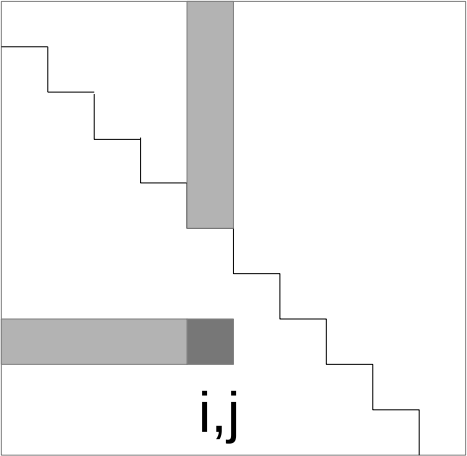
\includegraphics[width=.8\textwidth, keepaspectratio]{images/ch01/CMPP_elements_used_compute_sum_L.png}
		\label{Figure:theory->ICMPP->LUP->CMPP->sum-in-element-computation-dependance-L}
	\end{subfigure}%
	\begin{subfigure}{.5\textwidth}
		\centering
		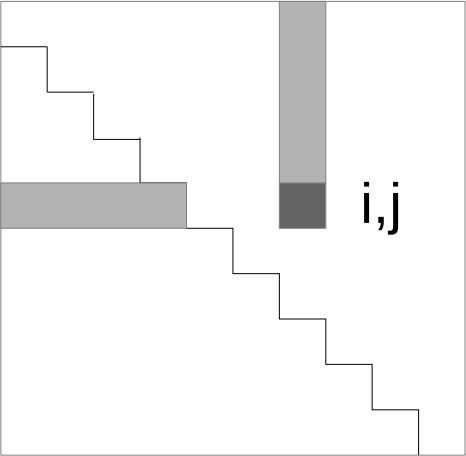
\includegraphics[width=.8\textwidth, keepaspectratio]{images/ch01/CMPP_elements_used_compute_sum_U.png}
		\label{Figure:theory->ICMPP->LUP->CMPP->sum-in-element-computation-dependance-U}
	\end{subfigure}
	\caption{Two examples of elements used (light gray squares) to compute the sum in the formula of elements $l_{i,j}$ and $u_{i,j}$ (dark gray squares).
		The lower triangle of the matrix consists of the corresponding elements of the lower triangle from $\mathbf{L}$ while the upper triangle consists of the corresponding elements of the upper triangle from $\mathbf{U}$.
		To compute the sum, only elements with indices in the interval $\left[1, \minp{i, j}\right)$, i.e., excluding the right boundary, are used in the element's row and column.
		Taken from \citetitle{Cejka2022} \cite{Cejka2022} and \citetitle{Chow2015} \cite{Chow2015}.
		}
	\label{Figure:theory->ICMPP->LUP->CMPP->sum-in-element-computation-dependance}
\end{figure}

In summary, an element in row $i$ and column $j$ is dependent on elements with indices $\left[1, \minp{i, j}\right)$ from its row and elements with indices $\left[1, \minp{i, j}\right)$ from its column.
This means that CMPP's algorithm is inherently sequential, which seemingly limits its potential for parallelization.

Thus far, the variation of CMPP discussed will either produce an exact solution in a finite amount of steps or, if the matrix is singular, it will fail.
In terms of numerical methods such a method is referred to as \textit{direct}.

An alternative group of methods to direct methods is known as iterative methods.
Unlike direct methods, iterative methods converge to a solution, but there is no guarantee that the exact solution will be obtained.
An example of an iterative variant of CMPP: \textit{Iterative Crout's Method with Partial Pivoting} (ICMPP) will be described in the next part.

\subsection{Iterative Crout's Method with Partial Pivoting (ICMPP)}\label{Subsection:theory->ICMPP->LUP->ICMPP}
Seeing as the potential for parallelization is seemingly limited for CMPP's algorithm, an alternative approach can be used.
One such alternative, put forward by \citename{Anzt2019}{author} in \citetitle{Anzt2019} \cite{Anzt2019}, involves using the formulas of CM in an iterative method.
Although the method proposed by the authors generates incomplete factorization, i.e., some nonzero elements are omitted during factorization, its principle can be extracted to create an iterative decomposition method that produces a complete factorization.
As detailed in \citetitle{Cejka2022} \cite{Cejka2022}, the complete-factorization approach converges to a sufficiently approximate solution of $\mathbf{A} = \mathbf{LU}$.
This approach, labeled as \textit{Iterative Crout's Method} (ICM), has been modified to include partial pivoting, thus creating \textit{Iterative Crout's Method with Partial Pivoting} (ICMPP).

The decomposition of matrix $\mathbf{A} \in \mathbb{R}^{n \times n} \left(n \in \mathbb{N}\right)$ into the product of matrices $\mathbf{L}, \mathbf{U} \in \mathbb{R}^{n \times n}$, and a permutation matrix $\mathbf{P} \in \left\{0,1\right\}^{n \times n}$ using ICMPP consists of the following steps \cite{Cejka2022}:

\begin{enumerate}
	\item Create an initial estimate of matrices $\mathbf{L}^{0}$ and $\mathbf{U}^{0}$ using $\mathbf{A}$:
		\begin{align}
			l_{i,j}^{0} & = a_{i,j} & u_{i,j}^{0} & = 0 \quad & i > j \nonumber\,, &  \\
			u_{i,j}^{0} & = a_{i,j} & l_{i,j}^{0} & = 0 \quad & i < j \nonumber\,, &  \\
			l_{i,j}^{0} & = a_{i,j} & u_{i,j}^{0} & = 1       & i = j \nonumber\,, &
		\end{align}
		and initialize $\mathbf{P}$ as the identity matrix.
	\item Denote the current iteration as $t \in \mathbb{N}$ and initialize it to 1.
	\item \label{Item:theory->ICMPP->LUP->ICMPP->algorithm-steps->compute-Lt}
		Compute $\mathbf{L}^{t}$ using Formula~\ref{Equation:theory->ICMPP->LUP->CMPP->lij}:
		\begin{align}
			l_{i,j}^{t} &= a_{i,j} - \sum_{k=1}^{j-1}l_{i,k}^{t-1}u_{k,j}^{t-1} &\quad i \geq j \nonumber\,.
		\end{align}
	\item \label{Item:theory->ICMPP->LUP->ICMPP->algorithm-steps->converge-lower-sections}
		Take the first $j \in \widehat{n}$ that satisfies the conditions $\left|l^{t-1}_{j, j} - l^{t}_{j, j}\right| \leq \epsilon_1$ (where $\epsilon_1$ denotes a tolerance, e.g., 0.001) and $\left|l^{t}_{j, j}\right| \leq \epsilon_2$, where $\epsilon_2$ denotes a \textit{pivoting tolerance}, e.g., 1e-5.
		In other words, find the first element on the main diagonal of $\mathbf{L}$ whose value is finalized and check if it requires pivoting according to the pivoting tolerance.
		In the context of this project, pivoting an element only when it is smaller than (or equal to) the pivoting tolerance is referred to as \textit{conditional partial pivoting}.
		If no such $j$ satisfies the conditions, proceed to Step~\ref{Item:theory->ICMPP->LUP->ICMPP->algorithm-steps->compute-Ut}.
		Then, \textit{iteratively converge} all elements in $\mathbf{L}^{t}$ below row $j$ from column 1 to column $j$ (including both boundaries), i.e., $l^{t}_{b, c}$ where $j < b \leq n$ and $1 \leq c \leq j$.
		In this context, \textit{iteratively converge} signifies to continue computing the mentioned elements using Formula~\ref{Equation:theory->ICMPP->LUP->CMPP->lij} until they all satisfy the condition $\left|l^{t-1}_{b, c} - l^{t}_{b, c}\right| \leq \epsilon_1$.
	\item \label{Item:theory->ICMPP->LUP->ICMPP->algorithm-steps->pivot-row}
		Pivot row $j$ (same as Step~\ref{Item:theory->ICMPP->LUP->CMPP->algorithm-steps->pivot-row-j} in the CMPP algorithm described on Page~\pageref{Item:theory->ICMPP->LUP->CMPP->algorithm-steps->pivot-row-j}):
		\begin{enumerate}
			\item \label{Item:theory->ICMPP->LUP->ICMPP->algorithm-steps->pivot-row->argmax}
				Find the index ($p$) of the element largest in absolute value in column $j$ from row $j$ to $n$:
				\begin{equation}
					p = \argmax_k \left\{ \left| l^{t}_{k, j} \right|: k=j,\dots, n \right\} \nonumber\,.
				\end{equation}
			\item \label{Item:theory->ICMPP->LUP->ICMPP->algorithm-steps->pivot-row->swap-rows}
				If $j$ is not equal to $p$, swap rows $j$ and $p$ in matrices $\mathbf{A}$, $\mathbf{L}^{t}$, $\mathbf{U}^{t}$, and $\mathbf{P}$.
			\item \label{Item:theory->ICMPP->LUP->ICMPP->algorithm-steps->pivot-row->singular-matrix-check}
				If $l^{t}_{j,j}$ is equal to 0, then the decomposition procedure has failed as the matrix is singular.
		\end{enumerate}
	\item \label{Item:theory->ICMPP->LUP->ICMPP->algorithm-steps->compute-Ut}
		Compute $\mathbf{U}^{t}$ using the values of $\mathbf{L}^{t}$ computed in earlier steps according to the formula provided in Equation~\ref{Equation:theory->ICMPP->LUP->CMPP->uij}:
		\begin{align}
			u_{i,j}^{t} &= \frac{1}{l_{i,i}^{t}} \left ( a_{i,j} - \sum_{k=1}^{i-1}l_{i,k}^{t}u_{k,j}^{t-1} \right ) &\quad i < j \nonumber\,.
		\end{align}
	\item \label{Item:theory->ICMPP->LUP->ICMPP->algorithm-steps->evaluate-convergence-rule}
		If the maximum absolute difference between $\mathbf{L}^{t-1}$ and $\mathbf{L}^{t}$, or between $\mathbf{U}^{t-1}$ and $\mathbf{U}^{t}$, exceeds tolerance $\epsilon_1$, then increment $t$ by 1 and return to Step~\ref{Item:theory->ICMPP->LUP->ICMPP->algorithm-steps->compute-Lt}.
	\item The algorithm has converged to an approximate solution of $\mathbf{A} = \mathbf{LUP}$, where $\mathbf{A}$  represents its original state before any potential changes occurred during this algorithm.
\end{enumerate}

While the instructions in Steps~\ref{Item:theory->ICMPP->LUP->ICMPP->algorithm-steps->compute-Lt} to \ref{Item:theory->ICMPP->LUP->ICMPP->algorithm-steps->evaluate-convergence-rule} must be performed consecutively, the operations in each step can be executed in parallel:

\begin{itemize}
	\item Step~\ref{Item:theory->ICMPP->LUP->ICMPP->algorithm-steps->compute-Lt} - The element $l^{t}_{i,j} \left(i, j \in \widehat{n}; n \in \mathbb{N}\right)$ is dependent only on elements from matrices $\mathbf{A}$, $\mathbf{L}^{t-1}$, and $\mathbf{U}^{t-1}$.
Since the values in the first matrix are constant - excluding the swapping of rows - and the last two matrices were set in the previous iteration, no elements from $\mathbf{L}^{t}$ are dependent on each other.
Thus, all elements $l^{t}_{i,j}$ can be computed simultaneously.
	\item Step \ref{Item:theory->ICMPP->LUP->ICMPP->algorithm-steps->converge-lower-sections} - The absolute-value conditions can be checked in parallel, and, similarly to Step~\ref{Item:theory->ICMPP->LUP->ICMPP->algorithm-steps->compute-Lt}, the iterative convergence is computed according to the same formula.
	\item Step \ref{Item:theory->ICMPP->LUP->ICMPP->algorithm-steps->pivot-row} - The $\max$ operation mentioned in Section~\ref{Subsection:theory->CUDA->parallel-reduction} can be adapted to suit the needs of $\argmax$ used in Step~\ref{Item:theory->ICMPP->LUP->ICMPP->algorithm-steps->pivot-row->argmax}.
While the swapping of elements in two rows can be performed in parallel, Steps~\ref{Item:theory->ICMPP->LUP->ICMPP->algorithm-steps->pivot-row->swap-rows} and \ref{Item:theory->ICMPP->LUP->ICMPP->algorithm-steps->pivot-row->singular-matrix-check} must be executed consecutively.
	\item Step \ref{Item:theory->ICMPP->LUP->ICMPP->algorithm-steps->compute-Ut} - The element $u^{t}_{i,j} \left(i, j \in \widehat{n}; n \in \mathbb{N}\right)$ is dependent only on elements from matrices $\mathbf{A}$, $\mathbf{L}^{t}$, and $\mathbf{U}^{t-1}$.
Matrices $\mathbf{A}$ and $\mathbf{U}^{t-1}$ were covered in the description of parallelization of Step~\ref{Item:theory->ICMPP->LUP->ICMPP->algorithm-steps->compute-Lt} and matrix $\mathbf{L}^{t}$ was finalized in Steps~\ref{Item:theory->ICMPP->LUP->ICMPP->algorithm-steps->compute-Lt} to \ref{Item:theory->ICMPP->LUP->ICMPP->algorithm-steps->pivot-row}.
Thus, since no elements from $\mathbf{U}^{t}$ are dependent on each other, they can be computed simultaneously.
	\item Step~\ref{Item:theory->ICMPP->LUP->ICMPP->algorithm-steps->evaluate-convergence-rule} - Since the evaluation of the convergence rule has no dependencies, it is entirely parallelizable.
\end{itemize}

Note that due to the nature of iterative methods, it is not possible to accurately predict the number of iterations needed to converge to an approximate solution.
Thus, the performance of ICMPP may heavily depend on the nonzero element structure of matrix $\mathbf{A}$.

To summarize, in Sections~\ref{Section:theory->GPUs} and \ref{Section:theory->CUDA} a high-performance parallel computing system was introduced in the form of Nvidia GPUs manageable by CUDA.
Then, in Section~\ref{Subsection:theory->ICMPP->LUP->ICMPP}, a parallelizable algorithm was presented.
The combination of the aforementioned parts will be the main focus of the following chapters.

\chapter*{Conclusion}				   	   % DO NOT TOUCH!
\addcontentsline{toc}{chapter}{Conclusion} % DO NOT TOUCH!

The objective of this thesis was to implement an iterative parallel LUP (Lower-Upper decomposition with Pivoting) algorithm, analyze its performance in BDDCML (multilevel Balancing Domain Decomposition by Constraints solver Library), and compare it to other established LUP implementations.

The first part of the thesis introduced the hardware of CPUs and GPUs, providing a basic understanding of their suitability for computations.
The specifications of recent GPUs were also presented to strengthen the theoretical foundation.
The relevant aspects of the software layer for code orchestration on Nvidia GPUs, CUDA, were then introduced, along with parallel computation concepts used in the implementation.
Finally, the theoretical foundation concluded with the introduction of LUP algorithms and their application in solving systems of equations.

Then, the implementation of the project that encompassed procedures related to solving systems of equations using LUP was presented.
Building upon the information presented in the first chapter, the implementations of the LUP procedures were detailed.
Additionally, the unit tests, which assured the quality of the implemented algorithms, were presented, along with the benchmarks that were later used to evaluate the performance of the implementations.

Finally, the procedures implemented in the project were compared to established CUDA libraries in terms of execution speed and accuracy of results on a state-of-the-art HPC cluster.
The comparison of performance was facilitated through two benchmarks.
The first benchmark - Decomposition benchmark - evaluated the raw performance of the procedures on a set of 50 matrices with varying characteristics.
The second benchmark - BDDCML benchmark - involved assessing the performance of the procedures as part of BDDCML.\\
The results of the Decomposition benchmark revealed that among the procedures implemented, the PCM\_8PP (Parallel Crout's Method with Partial Pivoting and $8^2$ threads in each one-dimensional CUDA thread block) decomposer exhibited the most consistent performance, while the ICM\_32PP (Iterative Crout's Method with Partial Pivoting and 32-by-32 CUDA thread blocks) decomposer showed suitability only for specific types of matrices.
However, both decomposers performed worse compared to the CusolverDnXgetrf procedure provided by CUDA.
The implemented solver, IS\_\textit{x}PP (Iterative Solver with Partial Pivoting and \textit{x}-by-8 CUDA thread blocks), was deemed unusable as it occasionally provided invalid results.\\
The second benchmark revealed that ICM\_32PP was able to compete with CUDA's cusolverDnXgetrf and MAGMA's magma\_dgetrf\_gpu.
Specifically, the relaxed processing tolerance of the iterative approach of ICM\_32PP allowed it to complete the benchmark at 90\% of the speed of magma\_dgetrf\_gpu.

As mentioned in Section~\ref{Subsection:comparing-decomposers-and-solvers->decomposition-project-benchmarks->decomposers-benchmark->accuracy-of-results-on-all-matrices}, using the maximum absolute difference between actual and expected results as a measure of accuracy has its limitations.
Furthermore, the time-consuming nature of the accuracy measurements restricted the number of matrices that could be included in the benchmark.
Therefore, future work could include developing a more suitable and efficient approach for measuring the accuracy of results.
This revised approach could also help elucidate the issues highlighted in Sections~\ref{Subsection:comparing-decomposers-and-solvers->decomposition-project-benchmarks->decomposers-benchmark->accuracy-of-results-on-all-matrices} and \ref{Subsection:comparing-decomposers-and-solvers->decomposition-project-benchmarks->solvers-benchmark->accuracy-of-results-on-all-matrices}.
Further areas of future improvement could include refining the algorithm of ICM\_\textit{x}PP based on the benchmark results, and implementing project-based enhancements, such as automated benchmarks and automated processing of their results.
These enhancements would significantly contribute to the overall efficiency and effectiveness of the project.

\printbibliography

\newpage 									% DO NOT TOUCH!
\addcontentsline{toc}{chapter}{Appendices}	% DO NOT TOUCH!
\appendix

\chapter{CMPP Implementation}\label{Appendix:CMPP-implementation}
The implementation of CMPP and the functions it uses are shown in Listing~\ref{Listing:CMPP-implementation-excerpt}.

\begin{lstlisting}[caption={Excerpt from the implementation of CMPP. The \code{pivotRowOfMatrix\_host()} function, presented below the \code{decompose()} method, is implemented in the parent class of \code{CroutMethod}: \code{BaseDecomposer}. Note that the code has been slightly modified for brevity. For example, the \code{swapRows\_host()} function has been omitted as it is a basic operation, and the checks for appropriate sizing of matrices/vectors have been removed.},label={Listing:CMPP-implementation-excerpt}]
template< typename Matrix, typename Vector >
void
CroutMethod::decompose( Matrix& LU, Vector& piv )
{
	using Real = typename Matrix::RealType;
	using Index = typename Matrix::IndexType;
	
	const Index& num_rows = LU.getRows();
	const Index& num_cols = LU.getColumns();
	
	// Pivoting tolerance
	const Real piv_tol = 1.0e-5;
	
	auto LU_view = LU.getView();
	auto piv_view = piv.getView();
	
	// Fill the pivoting vector with increments of 1 starting from 1 to num_rows.
	BaseDecomposer::setDefaultPivotingValues( piv );
	
	Index i, j, k, sum;
	
	for( j = 0; j < num_cols; ++j ) {
		for( i = j; i < num_rows; ++i ) {
			sum = 0;
			for( k = 0; k < j; ++k )
				sum = sum + LU_view( i, k ) * LU_view( k, j );
			
			LU_view( i, j ) = LU_view( i, j ) - sum;
		}
		
		if( TNL::abs( LU_view( j, j ) ) <= piv_tol ) {
			pivotRowOfMatrix_host( j, LU_view, num_rows, num_cols, piv_view );
			
			if( LU_view( j, j ) == 0 ) {
				// Last element in the matrix does not require pivoting as no elements are computed using it, i.e., division by zero cannot occur
				if( j != num_rows - 1 )
					throw Exceptions::MatrixSingular( "LU", j, j );
			}
		}
		
		for( i = j + 1; i < num_rows; ++i ) {
			sum = 0;
			for( k = 0; k < j; ++k )
				sum = sum + LU_view( j, k ) * LU_view( k, i );
			
			LU_view( j, i ) = ( LU_view( j, i ) - sum ) / LU_view( j, j );
		}
	}
}

template< typename Index, typename MatrixView, typename VectorView, typename Real = typename MatrixView::RealType >
std::pair< Real, Index >
pivotRowOfMatrix_host( const Index& j, MatrixView& M, const Index& num_rows, const Index& num_cols, VectorView& piv )
{
	// Find the row below the j-th row with max. value in the j-th column
	Real max = TNL::abs( M( j, j ) );  // or M(i,j)
	Index piv_row = j;
	
	for( Index i = j + 1; i < num_rows; ++i ) {
		Real zij = TNL::abs( M( i, j ) );
		if( zij > max ) {
			max = zij;
			piv_row = i;
		}
	}
	
	if( piv_row != j ) {  // exchange rows j, piv_row
		swapRows_host( M, j, piv_row, num_cols );
		piv( j ) = piv_row + 1;
	}
	
	return std::make_pair( max, piv_row );
}
\end{lstlisting}





\chapter{PCM\textit{x}PP Implementation}\label{Appendix:PCMxPP-implementation}
The implementation of PCM\textit{x}PP is shown in Listing~\ref{Listing:PCMxPP-implementation-excerpt}. Note that the kernels called in Listing~\ref{Listing:PCMxPP-implementation-excerpt} are shown separately in Listings~\ref{Listing:PCMxPP-implementation->kernels->column-compute-kernel} and \ref{Listing:PCMxPP-implementation->kernels->row-compute-kernel}.

\begin{lstlisting}[caption={Excerpt from the implementation of PCM\textit{x}PP. The template parameter \code{BLOCK\_SIZE} is equivalent to \textit{x} in PCM\textit{x}PP. On input, matrix \code{LU} is assumed to contain the values of $\mathbf{A}$, and \code{piv} is expected to be appropriately sized. Furthermore, unlike \code{LU}, \code{piv} is assumed to be allocated on the Host. The \code{pivotRowOfMatrix\_device()} function, presented below the \code{decompose()} method, is implemented in the parent class of \code{CroutMethod}: \code{BaseDecomposer}. Note that the code has been slightly modified for brevity. For example, the \code{swapRows\_device()} function has been omitted as it is a basic operation, and the checks for appropriate sizing of matrices/vectors have been removed.},label={Listing:PCMxPP-implementation-excerpt}]
template< const int BLOCK_SIZE >
template< typename Matrix, typename VecIndex, typename Device >
void
CroutMethod< BLOCK_SIZE >::decompose( Matrix& LU, Containers::RowOrderVector< VecIndex, Device >& piv )
{
	using Real = typename Matrix::RealType;
	using Index = typename Matrix::IndexType;
	
	const Index& num_rows = LU.getRows();
	const Index& num_cols = LU.getColumns();
	
	auto LU_view = LU.getView();
	auto piv_view = piv.getView();
	
	// Fill the pivoting vector with increments of 1 starting from 1 to num_rows.
	BaseDecomposer::setDefaultPivotingValues( piv );
	
	const Real piv_tol = 1.0e-5;
	
	constexpr int threads_perBlock = BLOCK_SIZE * BLOCK_SIZE;
	// Round to nearest higher multiple of threads_perBlock - only if threads_perBlock is a multiple of 2
	const Index num_cols_rounded = ( num_cols + threads_perBlock - 1 ) & -threads_perBlock;
	const Index blocks_perGrid = num_cols_rounded / threads_perBlock;
	
	for( Index diag = 0; diag < num_rows; ++diag ) {
		ColCompute_kernel<<< blocks_perGrid, threads_perBlock >>>( LU_view, diag, num_rows );
		
		if( TNL::abs( LU_view.getElement( diag, diag ) ) <= piv_tol ) {
			std::pair< Real, Index > max_elem = pivotRowOfMatrix_device< threads_perBlock >( diag, LU_view, num_rows, num_cols, piv_view );
			
			if( max_elem.first == 0 ) {
				// Last element does not require pivoting as no elements are computed using it - division by zero cannot occur for the last element
				if( diag != num_rows - 1 )
					throw Exceptions::MatrixSingular( "LU", diag, diag );
			}
		}
		
		RowCompute_kernel<<< blocks_perGrid, threads_perBlock >>>( LU_view, diag, num_cols );
	}
}

template< const int THREADS_PER_BLOCK,
		  typename Index,
		  typename MatrixView,
		  typename VectorView,
		  typename Real = typename MatrixView::RealType >
std::pair< Real, Index >
pivotRowOfMatrix_device( const Index& j, MatrixView& M, const Index& num_rows, const Index& num_cols, VectorView& piv )
{
	auto fetchAbsElement = [ = ] __cuda_callable__( Index row )
	{
		return abs( M( row, j ) );
	};
	std::pair< Real, Index > max_elem =
		TNL::Algorithms::reduceWithArgument< TNL::Devices::Cuda >( j, num_rows, fetchAbsElement, TNL::MaxWithArg{} );
	
	// Only need to swap rows if the pivoting row is different from j
	if( max_elem.second != j ) {
		swapRows_device< THREADS_PER_BLOCK >( M, j, max_elem.second, num_cols );
		piv( j ) = max_elem.second + 1;
	}
	
	return max_elem;
}
\end{lstlisting}

\begin{lstlisting}[caption={The implementation of the \code{ColCompute\_kernel()} kernel which computes one column of \code{LU}.},label={Listing:PCMxPP-implementation->kernels->column-compute-kernel}]
template< typename MatrixView, typename Index >
__global__
void
ColCompute_kernel( MatrixView LU, const Index col, const Index num_rows )
{
	using Real = typename MatrixView::RealType;
	// Offset threads to start from the diagonal element (including it)
	const Index row = blockIdx.x * blockDim.x + threadIdx.x + col;
	
	if( row >= num_rows )
		return;
	
	Real sum = 0;
	for( Index k = 0; k < col; ++k )
		sum += LU( row, k ) * LU( k, col );
	
	LU( row, col ) = LU( row, col ) - sum;
}
\end{lstlisting}

\begin{lstlisting}[caption={The implementation of the \code{RowCompute\_kernel()} kernel which computes one row of \code{LU}.},label={Listing:PCMxPP-implementation->kernels->row-compute-kernel}]
template< typename MatrixView, typename Index >
__global__
void
RowCompute_kernel( MatrixView LU, Index row, const Index num_cols )
{
	using Real = typename MatrixView::RealType;
	// Offset threads to start from element to the right of the diagonal element
	const Index col = blockIdx.x * blockDim.x + threadIdx.x + row + 1;
	
	if( col >= num_cols )
		return;
	
	Real sum = 0;
	for( Index k = 0; k < row; ++k )
		sum += LU( row, k ) * LU( k, col );
	
	LU( row, col ) = ( LU( row, col ) - sum ) / LU( row, row );
}
\end{lstlisting}





\chapter{ICM\textit{x}PP Implementation}\label{Appendix:ICMxPP-implementation}
The implementation of ICM\textit{x}PP is shown in Listing~\ref{Listing:ICMxPP-implementation-excerpt}. Note that the kernels called in Listing~\ref{Listing:ICMxPP-implementation-excerpt} are shown separately in Listings~\ref{Listing:implementation->decomposition-project->implemented-solutions->decomposers->ICMxPP->kernels->diagonal-compute}, \ref{Listing:implementation->decomposition-project->implemented-solutions->decomposers->ICMxPP->kernels->diagonal-assign}, \ref{Listing:ICMxPP-implementation->kernels->lower-section-compute}, and \ref{Listing:ICMxPP-implementation->kernels->right-section-compute}.

\begin{lstlisting}[caption={Excerpt from the implementation of ICM\textit{x}PP. The template parameter \code{BLOCK\_SIZE} is equivalent to \textit{x} in ICM\textit{x}PP. On input, matrix \code{A} is assumed to contain the values of $\mathbf{A}$, matrix \code{LU} is assumed to contain the initial estimate of the decomposition, and \code{piv} is expected to be appropriately sized and allocated on the Host. On output, matrix \code{LU} contains the values of matrices $\mathbf{L}$ and $\mathbf{U}$ in the format presented in Equation~\ref{Equation:implementation->decomposition-project->implemented-solutions->decomposers->CMPP}, and \code{piv} contains the row permutations. The \code{synchronizeStreams()} function is included below the \code{decompose()} method. The \code{pivotBadElement()} function is shown in Listing~\ref{Listing:ICMxPP-implementation-pivot-bad-element}. The code has been slightly modified for brevity, for example, the checks for appropriate sizing of matrices and vectors have been removed.},label={Listing:ICMxPP-implementation-excerpt}]
template< const int BLOCK_SIZE >
template< typename Matrix, typename Vector >
void
IterativeCroutMethod< BLOCK_SIZE >::decompose( Matrix& A, Matrix& LU, Vector& piv )
{
	using Real = typename Matrix::RealType;
	using Index = typename Matrix::IndexType;
	
	const Index num_rows = LU.getRows();
	const Index num_cols = LU.getColumns();
	
	// Matrix representing the next iteration
	Matrix LUnext;
	LUnext.setLike( LU );
	
	// Processing tolerance
	const Real process_tol = 0.0;
	// Pivoting tolerance
	const Real piv_tol = 1.0e-5;

	// Flag to indicate that the diagonal section has been processed
	TNL::Containers::Array< bool, TNL::Devices::Cuda > processed{ 1, false };
	
	// Fill the pivoting vector with increments of 1 starting from 1 to num_rows.
	BaseDecomposer::setDefaultPivotingValues( piv );
	
	// Determine the size of the section based on the dimensions of the matrix
	Index sec_size = min( max( num_cols / 10, (Index) 256 ), (Index) 1024 );
	sec_size = ( sec_size + BLOCK_SIZE - 1 ) / BLOCK_SIZE * BLOCK_SIZE;
	
	// CUDA grid configuration
	Index blocks = sec_size / BLOCK_SIZE;
	dim3 threads_perBlock( BLOCK_SIZE, BLOCK_SIZE );
	dim3 blocks_perGrid( blocks, blocks );
	
	// Allocate and initialize an array of stream handles to process sections in parallel
	const Index nonDiagSecs_perRow = TNL::ceil( (double) num_cols / (double) sec_size ) - 1;
	auto* streams = (cudaStream_t*) malloc( nonDiagSecs_perRow * sizeof( cudaStream_t ) );
	for( Index i = 0; i < nonDiagSecs_perRow; ++i )
		cudaStreamCreate( &( streams[ i ] ) );
	
	// Flags indicating the processing status of non-diagonal sections
	TNL::Containers::Array< bool, TNL::Devices::Cuda, Index > nonDiagSec_processed{ nonDiagSecs_perRow, false };
	TNL::Containers::Array< bool, TNL::Devices::Host, Index > nonDiagSec_processed_host{ nonDiagSecs_perRow, false };
	
	// Views are used from here on
	auto A_view = A.getView();
	auto LU_view = LU.getView();
	auto LUnext_view = LUnext.getView();
	auto piv_view = piv.getView();
	auto processed_view = processed.getView();
	auto nonDiagSec_processed_view = nonDiagSec_processed.getView();
	
	// Lambda for fetching the index of bad elements
	auto get_badEl_colIdxs = [ = ] __cuda_callable__( Index col ) -> Index
	{
		return abs( LU_view( col, col ) ) <= piv_tol ? col : num_cols;
	};
	
	// Diagonal section start and end
	Index dSec_start, dSec_end;
	// Non-diagonal section start, end, and id
	Index sec_start, sec_end, sec_id;
	Index badEl_idx;
	
	// Loop through the diagonal sections
	for( dSec_start = 0, dSec_end = min( num_cols, sec_size ); dSec_start < dSec_end; dSec_start += sec_size, dSec_end = min( num_cols, dSec_end + sec_size ) )
	{
		// Set the starting point of the search for the first bad element
		Index badEl_searchStart = dSec_start;
		
		do { // Process the diagonal section and the sections below it
			// Get next badEl_idx
			badEl_idx = TNL::Algorithms::reduce< TNL::Devices::Cuda >( badEl_searchStart, dSec_end, get_badEl_colIdxs, TNL::Min{}, num_cols );
			
			do {  // Process the diagonal section
				// Reset the processed flag
				processed_view.setElement( 0, true );
				
				// Compute the values up to and including the bad element
				DSecCompute_kernel< BLOCK_SIZE ><<< blocks_perGrid, threads_perBlock >>>( A_view, LU_view, LUnext_view, dSec_start, dSec_end, dSec_start, dSec_end, process_tol, processed_view, badEl_idx );
				
				// Assign the values computed for the next iteration
				DSecAssign_kernel<<< blocks_perGrid, threads_perBlock >>>( LU_view, LUnext_view, dSec_start, dSec_end, dSec_start, dSec_end, badEl_idx );
				
				// Check if a bad element is present between the previous bad element and the current bad element
				Index badEl_idx_new = TNL::Algorithms::reduce< TNL::Devices::Cuda >( badEl_searchStart, dSec_end, get_badEl_colIdxs, TNL::Min{}, num_cols );
				// If a bad element was detected before the current one -> set it as the new bad element
				if( badEl_idx_new < badEl_idx )
					badEl_idx = badEl_idx_new;
			} while( ! processed_view.getElement( 0 ) );
			
			// The Diagonal section contains processed values excluding the values to the bottom-right of the bad element
			// Compute the lower sections up to and including the column containing the bad element
			
			// Limit the number of threads used based on the number of columns that will be computed
			Index badEl_idx_cutoff = min( badEl_idx + 1, dSec_end );
			Index lSec_width_rounded = ( badEl_idx_cutoff - dSec_start + BLOCK_SIZE - 1 ) & -BLOCK_SIZE;
			dim3 lSec_blockPerGrid( TNL::max( lSec_width_rounded / BLOCK_SIZE, (Index) 1 ), blocks );
			
			// Default to false so that all kernels are run in the first iteration
			nonDiagSec_processed_view.setValue( false );
			
			do { // Process the lower sections in parallel
				nonDiagSec_processed_host = nonDiagSec_processed;
				nonDiagSec_processed_view.setValue( true );
				
				for( sec_start = dSec_end, sec_end = min( num_cols, dSec_end + sec_size ), sec_id = 0; sec_start < sec_end; sec_start += sec_size, sec_end = min( num_cols, sec_end + sec_size ), ++sec_id )
				{
					// Only compute sections that are not yet processed
					if( ! nonDiagSec_processed_host( sec_id ) ) {
						LSecCompute_kernel< BLOCK_SIZE ><<< lSec_blockPerGrid, threads_perBlock, 0, streams[ sec_id ] >>>( A_view, LU_view, LUnext_view, dSec_start, badEl_idx_cutoff, sec_start, sec_end, process_tol, nonDiagSec_processed_view, sec_id );
						
						NonDiagSecAssign_kernel<<< lSec_blockPerGrid, threads_perBlock, 0, streams[ sec_id ] >>>( LU_view, LUnext_view, dSec_start, badEl_idx_cutoff, sec_start, sec_end );
					}
				}
				// Wait until all sections have been computed in this iteration
				synchronizeStreams( streams, nonDiagSecs_perRow );
			} while( ! TNL::Algorithms::reduce( nonDiagSec_processed_view, TNL::LogicalAnd{} ) );
			
			// Pivot the bad element
			pivotBadElement< BLOCK_SIZE >( A_view, LU_view, piv_view, badEl_idx, num_rows, num_cols, badEl_searchStart, piv_tol );
			
		} while( badEl_idx < dSec_end - 1 );
		
		nonDiagSec_processed_view.setValue( false );
		
		// Process sections to the right of the diagonal section in parallel
		// At this point there are no bad elements in the diagonal section
		do {
			nonDiagSec_processed_host = nonDiagSec_processed;
			nonDiagSec_processed_view.setValue( true );
			
			// Launch kernels for all sections below the diagonal section - each section has its stream
			for( sec_start = dSec_end, sec_end = min( num_cols, dSec_end + sec_size ), sec_id = 0; sec_start < sec_end; sec_start += sec_size, sec_end = min( num_cols, sec_end + sec_size ), ++sec_id )
			{
				// Only compute sections that are not yet processed
				if( ! nonDiagSec_processed_host( sec_id ) ) {
					RSecCompute_kernel< BLOCK_SIZE ><<< blocks_perGrid, threads_perBlock, 0, streams[ sec_id ] >>>( A_view, LU_view, LUnext_view, sec_start, sec_end, dSec_start, dSec_end, process_tol, nonDiagSec_processed_view, sec_id );
					
					NonDiagSecAssign_kernel<<< blocks_perGrid, threads_perBlock, 0, streams[ sec_id ] >>>( LU_view, LUnext_view, sec_start, sec_end, dSec_start, dSec_end );
				}
			}
			// Wait until all sections have been computed in this iteration
			synchronizeStreams( streams, nonDiagSecs_perRow );
		} while( ! TNL::Algorithms::reduce( nonDiagSec_processed_view, TNL::LogicalAnd{} ) );
	}
	
	// Release resources
	for( Index i = 0; i < nonDiagSecs_perRow; ++i )
		cudaStreamDestroy( streams[ i ] );
	
	free( streams );
}

void
synchronizeStreams( cudaStream_t* streams, const int num_streams )
{
	for( int i = 0; i < num_streams; i++ )
		cudaStreamSynchronize( streams[ i ] );
}
\end{lstlisting}

\begin{lstlisting}[caption={The definition of the \code{pivotBadElement()} function which is responsible for pivoting a bad element found in column \code{j} of the main diagonal. The \code{pivotRowOfMatrices\_device()} function, presented below the \code{pivotBadElement()} function, is implemented in the parent class of \code{IterativeCroutMethod}: \code{BaseDecomposer}. Note that the variant of the \code{swapRows\_device()} function presented in the \code{pivotRowOfMatrices\_device()} swaps the rows in two matrices.},label={Listing:ICMxPP-implementation-pivot-bad-element}]
template< const int BLOCK_SIZE, typename MatrixView, typename VectorView, typename Index, typename Real >
void
pivotBadElement( MatrixView& A, MatrixView& LU, VectorView& piv, const Index& j, const Index& num_rows, const Index& num_cols, Index& badEl_searchStart, const Real& piv_tol )
{
	// The last element of the matrix does not require pivoting as no elements are computed using it, i.e., division by zero cannot occur for the last element
	if( j >= num_cols - 1 ) {
		return;
	}
	
	std::pair< Real, Index > max_elem = pivotRowOfMatrices_device< BLOCK_SIZE * BLOCK_SIZE >( j, A, LU, num_rows, num_cols, piv );
	
	if( max_elem.first == 0 ) {
		// The current bad element in the main diagonal is zero even after pivoting -> Decomposition failed
		throw Exceptions::MatrixSingular( "LU", j, j );
	}
	else if( max_elem.first <= piv_tol ) {
		// The value at the index of the bad element is smaller than the pivoting tolerance, however, it is not zero, so the computation can continue
		// Search for the next bad element after this one
		badEl_searchStart = j + 1;
	}
}

template< const int THREADS_PER_BLOCK, typename Index, typename MatrixView, typename VectorView, typename Real = typename MatrixView::RealType >
std::pair< Real, Index >
pivotRowOfMatrices_device( const Index& j, MatrixView& A, MatrixView& M, const Index& num_rows, const Index& num_cols, VectorView& piv )
{
	auto fetchAbsElement = [ = ] __cuda_callable__( Index row )
	{
		return abs( M( row, j ) );
	};
	
	std::pair< Real, Index > max_elem = TNL::Algorithms::reduceWithArgument< TNL::Devices::Cuda >( j, num_rows, fetchAbsElement, TNL::MaxWithArg{} );
	
	// Only need to swap rows if the pivoting row is different from j
	if( max_elem.second != j ) {
		swapRows_device< THREADS_PER_BLOCK >( A, M, j, max_elem.second, num_cols );
		piv( j ) = max_elem.second + 1;
	}
	
	return max_elem;
}
\end{lstlisting}

\begin{lstlisting}[caption={The implementation of the \code{LSecCompute\_kernel()} kernel which computes one iteration of a lower section. Note that the matrices, vectors, and arrays are passed using their views, and the scalar values are copied to the local memory of each thread.},label={Listing:ICMxPP-implementation->kernels->lower-section-compute}]
template< const int BLOCK_SIZE, typename ConstMatrixView, typename MatrixView, typename BoolArrayView, typename Index, typename Real >
__global__
void
LSecCompute_kernel( const ConstMatrixView A, MatrixView LU, MatrixView LUnext, const Index sec_start_col, const Index sec_end_col, const Index sec_start_row, const Index sec_end_row, const Real process_tol, BoolArrayView processed, const Index sec_id )
{
	Index ty = threadIdx.y;
	Index tx = threadIdx.x;
	
	// Each thread computes one element (row, col)
	Index row = blockIdx.y * blockDim.y + ty + sec_start_row;
	Index col = blockIdx.x * blockDim.x + tx + sec_start_col;
	
	// Set the IDs of threads that overreach the bounds to the closest boundary
	Index max_col = sec_end_col - 1;
	Index max_row = sec_end_row - 1;
	Index row_adj = min( row, max_row );
	Index col_adj = min( col, max_col );
	
	// Offset the smallest index of the thread's element by BLOCK_SIZE to allow for loop unrolling
	// In a lower section, the column index is always smaller
	Index min_row_col = col_adj - BLOCK_SIZE;
	
	__shared__ Real L_block[ BLOCK_SIZE ][ BLOCK_SIZE ];
	__shared__ Real U_block[ BLOCK_SIZE ][ BLOCK_SIZE ];
	
	Index i, k; Real sum = 0;
	
	// Compute the sum needed for the element (row, col) by loading blocks of elements from global to shared memory and multiplying them
	for( i = 0; i <= min_row_col; i += BLOCK_SIZE ) {
		L_block[ ty ][ tx ] = LU( row_adj, i + tx );
		U_block[ ty ][ tx ] = LU( i + ty, col_adj );
		
		__syncthreads();
		
		#pragma unroll( BLOCK_SIZE )
		for( k = 0; k < BLOCK_SIZE; ++k )
			sum += L_block[ ty ][ k ] * U_block[ k ][ tx ];
		__syncthreads();
	}
	
	// Loops are unrolled by multiples of BLOCK_SIZE and the remaining elements are computed separately
	L_block[ ty ][ tx ] = LU( row_adj, min( i + tx, max_col ) );
	U_block[ ty ][ tx ] = LU( min( i + ty, max_row ), col_adj );
	
	__syncthreads();
	
	// Terminate threads that overreach the bounds as they have served their purpose of reading data
	if( row >= sec_end_row || col >= sec_end_col )
		return;
	
	for( k = 0; k < tx; ++k )
		sum += L_block[ ty ][ k ] * U_block[ k ][ tx ];
	
	// Formula for L
	sum = A( row, col ) - sum;
	
	// Check if the element (row, col) has been processed
	// Read LU( row, col ) from shared memory instead of global memory
	if( abs( L_block[ ty ][ tx ] - sum ) > process_tol )
		processed( sec_id ) = false;
	
	// Assign the element for the next iteration
	LUnext( row, col ) = sum;
}
\end{lstlisting}

\begin{lstlisting}[caption={The implementation of the \code{RSecCompute\_kernel()} kernel which computes one iteration of a right section.},label={Listing:ICMxPP-implementation->kernels->right-section-compute}]
template< const int BLOCK_SIZE, typename ConstMatrixView, typename MatrixView, typename BoolArrayView, typename Index, typename Real >
__global__
void
RSecCompute_kernel( const ConstMatrixView A, MatrixView LU, MatrixView LUnext, const Index sec_start_col, const Index sec_end_col, const Index sec_start_row, const Index sec_end_row, const Real process_tol, BoolArrayView processed, const Index sec_id )
{
	Index tx = threadIdx.x;
	Index ty = threadIdx.y;
	
	// Each thread computes one element (row, col)
	Index row = blockIdx.y * blockDim.y + ty + sec_start_row;
	Index col = blockIdx.x * blockDim.x + tx + sec_start_col;
	
	// Set the IDs of threads that overreach the bounds to the closest boundary
	Index max_col = sec_end_col - 1;
	Index max_row = sec_end_row - 1;
	Index row_adj = min( row, max_row );
	Index col_adj = min( col, max_col );
	
	// Offset the smallest index of the thread's element by BLOCK_SIZE to allow for loop unrolling
	// In a right section, the row index is always smaller
	Index min_row_col = row_adj - BLOCK_SIZE;
	
	__shared__ Real L_block[ BLOCK_SIZE ][ BLOCK_SIZE ];
	__shared__ Real U_block[ BLOCK_SIZE ][ BLOCK_SIZE ];
	
	Index i, k; Real sum = 0;
	
	// Compute the sum needed for the element (row, col) by loading blocks of elements from global to shared memory and multiplying them
	for( i = 0; i <= min_row_col; i += BLOCK_SIZE ) {
		L_block[ ty ][ tx ] = LU( row_adj, i + tx );
		U_block[ ty ][ tx ] = LU( i + ty, col_adj );
		
		__syncthreads();
		
		#pragma unroll( BLOCK_SIZE )
		for( k = 0; k < BLOCK_SIZE; ++k )
			sum += L_block[ ty ][ k ] * U_block[ k ][ tx ];
		__syncthreads();
	}
	
	// Loops are unrolled by multiples of BLOCK_SIZE and the remaining elements are computed separately
	L_block[ ty ][ tx ] = LU( row_adj, min( i + tx, max_col ) );
	U_block[ ty ][ tx ] = LU( min( i + ty, max_row ), col_adj );
	
	__syncthreads();
	
	// Terminate threads that overreach the bounds as they have served their purpose of reading data
	if( row >= sec_end_row || col >= sec_end_col )
		return;
	
	for( k = 0; k < ty; ++k )
		sum += L_block[ ty ][ k ] * U_block[ k ][ tx ];
	
	// Formula for U
	// Do not check for division by zero as this kernel assumes that no bad element is present in the diagonal section
	sum = ( A( row, col ) - sum ) / LU( row, row );
	
	// Check if the element (row, col) has been processed
	// Read LU( row, col ) from shared memory instead of global memory
	if( abs( U_block[ ty ][ tx ] - sum ) > process_tol )
		processed( sec_id ) = false;
	
	// Assign the element for the next iteration
	LUnext( row, col ) = sum;
}
\end{lstlisting}

\begin{lstlisting}[caption={The implementation of the \code{NonDiagSecAssign\_kernel()} kernel that assigns values of the next iteration to the matrix representing the current iteration.},label={Listing:ICMxPP-implementation->kernels->nondiagonal-assign}]
template< typename MatrixView, typename Index >
__global__
void
NonDiagSecAssign_kernel( MatrixView LU, MatrixView LUnext, const Index sec_start_col, const Index sec_end_col, const Index sec_start_row, const Index sec_end_row )
{
	Index row = blockIdx.y * blockDim.y + threadIdx.y + sec_start_row;
	Index col = blockIdx.x * blockDim.x + threadIdx.x + sec_start_col;
	
	if( row >= sec_end_row || col >= sec_end_col )
		return;
	
	LU( row, col ) = LUnext( row, col );
}
\end{lstlisting}





\chapter{SSPP Implementation}\label{Appendix:SSPP-implementation}
The implementation of SSPP is shown in Listing~\ref{Listing:SSPP-implementation-excerpt}.

\begin{lstlisting}[caption={Excerpt from the implementation of SSPP. The code has been slightly modified for brevity, for example, the checks for appropriate sizing of matrices and vectors have been removed.},label={Listing:SSPP-implementation-excerpt}]
template< typename Matrix, typename Vector >
void
SequentialSolver::solve( const Matrix& LU, Matrix& X, const Vector& piv )
{
	using Real = typename Matrix::RealType;
	using Device = TNL::Devices::Host;
	using Index = typename Matrix::IndexType;
	
	const Index num_rows = LU.getRows();
	const Index num_cols = LU.getColumns();
	
	const Index nrhs = X.getColumns();
	TNL::Containers::Vector< Real, Device, Index > sum( nrhs );
	
	// Solve (LU)X = B, where X holds the values of B on input
	
	// Order Matrix X according to vec
	if( ! piv.empty() ) {
		Decomposers::BaseDecomposer::orderMatrixAccordingTo( X, piv );
	}
	
	// Just to keep the original labels in the loops for clarity
	auto X_view = X.getView();
	auto Y_view = X.getView();
	auto B_view = X.getView();
	
	auto LU_view = LU.getConstView();
	auto sum_view = sum.getView();
	
	// Forward substitution: LY = B
	for( Index i = 0; i < num_rows; ++i ) {
		sum_view.setValue( 0 );
		for( Index j = 0; j < i; ++j ) {
			// sum = sum + LU( i, j ) * Y( j );
			auto y_row = Y_view.getRow( j );
			auto rhsSum = [ = ] __cuda_callable__( Index rhs ) mutable
			{
				sum_view( rhs ) = sum_view( rhs ) + LU_view( i, j ) * y_row.getValue( rhs );
			};
			TNL::Algorithms::parallelFor< Device >( Index{ 0 }, nrhs, rhsSum );
		}
		// Y( i ) = ( B( i ) - sum ) / LU( i, i );
		auto y_row = Y_view.getRow( i );
		auto b_row = B_view.getRow( i );
		auto ySet = [ = ] __cuda_callable__( Index rhs ) mutable
		{
			y_row.setValue( rhs, ( b_row.getValue( rhs ) - sum_view( rhs ) ) / LU_view( i, i ) );
		};
		TNL::Algorithms::parallelFor< Device >( Index{ 0 }, nrhs, ySet );
	}
	
	// Backward substitution: UX = Y
	for( Index i = num_rows - 1; i >= 0; --i ) {
		sum_view.setValue( 0 );
		for( Index j = i + 1; j < num_cols; ++j ) {
			// sum = sum + LU( i, j ) * X( j );
			auto x_row = X_view.getRow( j );
			auto rhsSum = [ = ] __cuda_callable__( Index rhs ) mutable
			{
				sum_view( rhs ) = sum_view( rhs ) + LU_view( i, j ) * x_row.getValue( rhs );
			};
			TNL::Algorithms::parallelFor< Device >( Index{ 0 }, nrhs, rhsSum );
		}
		// X( i ) = Y( i ) - sum;		
		auto x_row = X_view.getRow( i );
		auto y_row = Y_view.getRow( i );
		auto xSet = [ = ] __cuda_callable__( Index rhs ) mutable
		{
			x_row.setValue( rhs, y_row.getValue( rhs ) - sum_view( rhs ) );
		};
		TNL::Algorithms::parallelFor< Device >( Index{ 0 }, nrhs, xSet );
	}
}
\end{lstlisting}




\chapter{IS\textit{x}PP Implementation}\label{Appendix:ISxPP-implementation}
The implementation of IS\_\textit{x}PP is shown in Listing~\ref{Listing:ISxPP-implementation-excerpt}. Note that the kernels called in Listing~\ref{Listing:ISxPP-implementation-excerpt} are shown separately in Listings~\ref{Listing:ISxPP-implementation->kernels->forward-substitution}, \ref{Listing:ISxPP-implementation->kernels->backward-substitution}, and \ref{Listing:ISxPP-implementation->kernels->matrix-assign}.

\begin{lstlisting}[caption={Excerpt from the implementation of IS\_\textit{x}PP. The code has been slightly modified for brevity, for example, the checks for appropriate sizing of matrices and vectors have been removed. Note that the CUDA thread blocks used in the implementation are larger in the 1st dimension. Threads adjacent in the 1st dimension are assigned to neighboring elements in the same column since the matrices are stored in column-major order on the GPU. In other words, to mitigate misaligned global memory access, the 1st dimension of threads is used to access elements in a single column and the 2nd dimension is used to differentiate between right-hand sides.},label={Listing:ISxPP-implementation-excerpt}]
template< const int THREADS_PER_BLOCK >
template< typename Matrix, typename Vector >
void
IterativeSolver< THREADS_PER_BLOCK >::solve( const Matrix& LU, Matrix& X, const Vector& piv )
{
	using Real = typename Matrix::RealType;
	using Index = typename Matrix::IndexType;
	
	const Index num_rows = LU.getRows();
	const Index num_cols = LU.getColumns();
	
	const Index nrhs = X.getColumns();
	
	// Solve (LU)X = B, where X holds the values of B on input
	
	// Order Matrix X according to vec
	if( ! piv.empty() ) {
		Decomposers::BaseDecomposer::orderMatrixAccordingTo( X, piv );
	}
	
	Matrix Xnext;
	Xnext.setLike( X );
	
	Matrix Y;
	Y.setLike( X );
	Matrix Ynext;
	Ynext.setLike( Y );
	
	// X holds the values of B on input
	auto X_view = X.getView();
	auto Y_view = Y.getView();
	auto B_view = X.getView();
	auto Xnext_view = Xnext.getView();
	auto Ynext_view = Ynext.getView();
	
	auto LU_view = LU.getConstView();
	
	// Flag to indicate that a section has been processed
	TNL::Containers::Array< bool, TNL::Devices::Cuda > processed{ 1, true };
	auto processed_view = processed.getView();
	const Real process_tol = 0.0;
	
	// Round to nearest higher multiple of THREADS_PER_BLOCK
	Index num_rows_rounded = ( num_rows + THREADS_PER_BLOCK - 1 ) / THREADS_PER_BLOCK * THREADS_PER_BLOCK;
	
	// Number of right-hand sides is usually small
	const Index BLOCK_SIZE_y = 8;
	const Index nrhs_rounded = ( nrhs + BLOCK_SIZE_y - 1 ) / BLOCK_SIZE_y * BLOCK_SIZE_y;
	
	const Index blocks_perGrid_x = num_rows_rounded / THREADS_PER_BLOCK;
	const Index blocks_perGrid_y = nrhs_rounded / BLOCK_SIZE_y;
	
	dim3 threads_perBlock( THREADS_PER_BLOCK, BLOCK_SIZE_y );
	dim3 blocks_perGrid( blocks_perGrid_x, blocks_perGrid_y );
	
	// Forward substitution: LY = B
	do {
		processed_view.setElement( 0, true );
		FowardSubst_kernel<<< blocks_perGrid, threads_perBlock >>>( LU_view, Y_view, Ynext_view, B_view, num_rows, nrhs, processed_view, process_tol );
		
		MtxAssign_kernel<<< blocks_perGrid, threads_perBlock >>>( Y_view, Ynext_view, num_rows, nrhs );
	} while( ! processed_view.getElement( 0 ) );
	
	// Backward substitution: UX = Y
	do {
		processed_view.setElement( 0, true );
		BackwardSubst_kernel<<< blocks_perGrid, threads_perBlock >>>( LU_view, X_view, Xnext_view, Y_view, num_rows, num_cols, nrhs, processed_view, process_tol );

		MtxAssign_kernel<<< blocks_perGrid, threads_perBlock >>>( X_view, Xnext_view, num_rows, nrhs );
	} while( ! processed_view.getElement( 0 ) );
}
\end{lstlisting}

\begin{lstlisting}[caption={The implementation of the \code{FowardSubst\_kernel()} kernel which computes one forward-substitution iteration.},label={Listing:ISxPP-implementation->kernels->forward-substitution}]
template< typename ConstMatrixView, typename MatrixView, typename Index, typename BoolArrayView, typename Real >
__global__
void
FowardSubst_kernel( const ConstMatrixView LU, MatrixView Y, MatrixView Ynext, const MatrixView B, const Index num_rows, const Index nrhs, BoolArrayView processed, const Real process_tol )
{
	// Each thread computes one element (row, rhs)
	const Index row = blockIdx.x * blockDim.x + threadIdx.x;
	const Index rhs = blockIdx.y * blockDim.y + threadIdx.y;
	
	// Terminate threads that overreach matrix bounds
	if( row >= num_rows || rhs >= nrhs )
		return;
	
	Real sum = 0;
	
	for( Index j = 0; j < row; ++j )
		sum = sum + LU( row, j ) * Y( j, rhs );
	
	sum = ( B( row, rhs ) - sum ) / LU( row, row );
	
	// Check if the element (row, rhs) has been processed
	if( abs( Y( row, rhs ) - sum ) > process_tol )
		processed( 0 ) = false;
	
	// Assign the element for the next iteration
	Ynext( row, rhs ) = sum;
}
\end{lstlisting}

\begin{lstlisting}[caption={The implementation of the \code{BackwardSubst\_kernel()} kernel which computes one backward-substitution iteration.},label={Listing:ISxPP-implementation->kernels->backward-substitution}]
template< typename ConstMatrixView, typename MatrixView, typename BoolArrayView, typename Real, typename Index >
__global__
void
BackwardSubst_kernel( const ConstMatrixView LU, MatrixView X, MatrixView Xnext, const MatrixView Y, const Index num_rows, const Index num_cols, const Index nrhs, BoolArrayView processed, const Real process_tol )
{
	// Each thread computes one element (row, rhs)
	const Index row = blockIdx.x * blockDim.x + threadIdx.x;
	const Index rhs = blockIdx.y * blockDim.y + threadIdx.y;
	
	// Terminate threads that overreach matrix bounds
	if( row >= num_rows || rhs >= nrhs )
		return;
	
	Real sum = 0;
	
	for( Index j = row + 1; j < num_cols; ++j )
		sum = sum + LU( row, j ) * X( j, rhs );
	
	sum = Y( row, rhs ) - sum;
	
	// Check if the element (row, rhs) has been processed
	if( abs( X( row, rhs ) - sum ) > process_tol )
		processed( 0 ) = false;
	
	// Assign the element for the next iteration
	Xnext( row, rhs ) = sum;
}
\end{lstlisting}

\begin{lstlisting}[caption={The implementation of the \code{MtxAssign\_kernel()} kernel that assigns values of the next iteration to the matrix representing the current iteration.},label={Listing:ISxPP-implementation->kernels->matrix-assign}]
template< typename MatrixView, typename Index >
__global__
void
MtxAssign_kernel( MatrixView M, MatrixView Mnext, const Index num_rows, const Index num_cols )
{
	// Each thread assigns one element (row, rhs)
	const Index row = blockIdx.x * blockDim.x + threadIdx.x;
	const Index rhs = blockIdx.y * blockDim.y + threadIdx.y;
	
	// Terminate threads that overreach matrix bounds
	if( row >= num_rows || rhs >= num_cols )
		return;
	
	M( row, rhs ) = Mnext( row, rhs );
}
\end{lstlisting}

% Write out all citation in the bibliography - even if they're not cited in the text
% This must be last so that citation numbering depends on the order the entries were cited in. Then the remaining non-cited entries can be printed in the bibliography
\nocite{*}
	
\end{document}